\documentclass[a4paper,10pt]{article}
\usepackage[utf8]{inputenc}
\input{auxiliar/tex/encabezado.tex}
\input{auxiliar/tex/tikzlibrarybayesnet.code.tex}
\newif\ifen
\newif\ifes
\newcommand{\en}[1]{\ifen#1\fi}
\newcommand{\es}[1]{\ifes#1\fi}
\entrue

\newcommand{\E}{\en{S}\es{E}}
\newcommand{\A}{\en{E}\es{A}}
\newcommand{\Ee}{\en{s}\es{e}}
\newcommand{\Aa}{\en{e}\es{a}}



\newtheorem{conclution}{\en{Conclution}\es{Conclusión}}%[section]
\newtheorem{objective}{\en{Objective}\es{Objetivo}}%[section]



%opening
\title{Multilevel selection in causal nonergodic process: the evolutionary advantage of cooperation and especialization.}
\author{Gustavo Landfried}

\begin{document}

\maketitle

\begin{abstract}
\en{In the last third of the universe's history, a simple self-replicating organization of matter emerged on earth. }%
\es{En el último tercio de la historia del universo surgió en la tierra una organización de la materia simple capaz de autoreplicarse. }%
%
\en{The growth of these lineages followed multiplicative and noisy processes: sequences of survival and reproduction rates. }%
\es{El crecimiento de estos linajes siguieron procesos multiplicativos y ruidosos: secuencias de tasas de supervivencia y reproducción. }%
%
\en{The current complexity of life is the consequence of a series of evolutionary transitions in which entities capable of self-replication after the transition become part of higher level cooperative units. }%
\es{La complejidad actual de la vida es consecuencia de una serie de transiciones evolutivas en las que entidades capaces de autoreplicación luego de la transición pasan a formar parte de unidades cooperativas de nivel superior. }%
%
\en{How to explain this permanent tendency of life in favor of cooperative aggregation and specialization? }%
\es{¿Cómo se explica esta tendencia permanente de la vida en favor de la agregación cooperativa y la especialización? }%

% Parrafo

\en{Recently Ole Peters has shown that, as a consequence of the non-ergodicity of multiplicative processes, fluctuations have a negative effect on individual growth rates, which can be reduced through mutual cooperation, leading to an increase in the long-term growth rates of all individuals. }%
\es{Recientemente Ole Peters ha mostrado que, como consecuencia de la no-ergodicidad de los procesos multiplicativos, las fluctuaciones tienen un efecto negativo en las tasas de crecimiento individuales, las cuales pueden ser reducidas a través de la mutua cooperación, produciendo un aumento de la tasas de crecimiento a largo plazo de todos los individuos. }%
%
\en{Ole Peters believs that the increase in the growth rate is sufficient argument to demonstrate the evolutionary advantage of cooperation, which he proposes as the main explanation for evolutionary transitions. }%
\es{Ole Peters considera que el aumento de la tasa de crecimiento es argumento suficiente para demostrar la ventaja evolutiva de la cooperación, lo que propone como principal explicación de las transiciones evolutivas. }%
%
\en{However, he does not consider the problem of defection, who says ``our cooperators are unable to break the cooperative pact''. }%
\es{Sin embargo no considera el problema de la deserción, quien dice ``our cooperators are unable to break the cooperative pact''. }%

% Parrafo

\en{To explain evolutionary transitions, it is necessary to demonstrate the evolutionary advantage of cooperation in the presence of defection, but also the advantage of specialization. }%
\es{Para explicar las transiciones evolutivas es necesario demostrar la ventaja evolutiva de la cooperación en presencia de deserción, pero también la ventaja de la especiliazación. }%
%
\en{For this purpose it is necessary to consider selection at both the individual and group level. }%
\es{Para este propósito es necesario considerar selección tanto a nivel individual como a nivel grupal. }%
%
\en{The co-author of the concept of evolutionary transitions (Szathmary) recently proposed to analyze the evolution of populations subject to multilevel selection by means of Bayesian hierarchical models, making use of the isomorphism between evolutionary theory and Bayesian inference. }%
\es{El co-autor del concepto de transiciones evolutivas (Szathmary) propuso recientemente analizar la evolución de las poblaciones sujetas a selección multinivel mediante modelos jerárquicos bayesianos, haciendo uso del isomorfismo entre las teoría de la evolución y la inferencia bayesiana. }%
%
\en{However, beyond the proposal, the authors of this article (Czegel et al) fail to offer a model that represents multilevel selection, their examples are only pictorial. }%
\es{Sin embargo, más allá de la propuesta, los autores de este artículo (Czegel et al) no logran ofrecer un modelo que represente selección multinivel, sus ejemplos son sólo pictóricos. }%

% Parrafo

\en{In this paper we include the problem of defection, and show that while resource-avoidance strategies can invade entirely cooperative groups by natural selection, such behavior at the same time increases their own individual fluctuations, reducing their own long-term growth rate without the need to introduce penalties. }%
\es{En este trabajo incluimos el problema de la deserción, y mostramos que, si bien las estrategias que evitan compartir recursos pueden invadir por selección natural grupos enteramente cooperadores, tal comportamiento aumenta al mismo tiempo sus propias fluctuaciones individuales, reduciendo su propia tasa de crecimiento a largo plazo sin necesidad de introducir castigos. }%
%
\en{That is, contrary to the belief established since the mid-20th century in economics, we show that the dynamics of common goods under multiplicative processes cannot be represented by a prisoner's dilemma payoff matrix. }%
\es{Es decir, en contra de la creencia establecida que en economía se tiene desde mediados del siglo 20, mostramos que los dinámicas de bienes comunes bajo procesos multiplicativos no puede representarse mediante una matriz de pagos del dilema del prisionero. }%
%
\en{Using the equivalence between multilevel selection and inference in Bayesian hierarchical models, we show that unconditionally cooperative strategies, without being evolutionarily stable within groups, are evolutionarily favored through group selection. }%
\es{Utilizando la equivalencia entre la selección multinivel y la inferencia en modelos jerárquicos bayesianos, mostramos que las estrategias incondicionalmente cooperadoras, sin ser evolutivamente estables al interior de los grupos, se ven favorecidas evolutivamente a través de la selección grupal. }%
%
\en{And we also show that strategies that are individually poorly adapted to the environment (specialists), once cooperation emerges, manage to outperform both individually well-adapted strategies (generalists), as well as their cooperative groups of infinite size. }%
\es{Y mostramos además que, una vez que la cooperación emerge, las estrategias individualmente mal adaptadas al ambiente (especialistas) consigen superar tanto a las estrategias bien adaptas individualmemte (generalistas), como a sus grupos cooperativos de tamaño infinito. }%

% Parrafo

\en{Extending the argument proposed by Ole Peters by means of the methodology proposed by the co-author of the concept of evolutionary transitions, we show that the evolutionary advantage of cooperation and specialization is a consequence of the non-ergodicity of the multiplicative processes that govern the growth of life, so that this must be considered the first cause of major evolutionary transitions. }%
\es{Extendiendo el argumento propuesto por Ole Peters mediante la metodología propuesta por el co-autor del concepto de transiciones evolutivas, demostramos que la ventaja evolutiva de la cooperación y de la especialización es consecuencia de la no-ergodicidad de los procesos multiplicativos que gobiernan el crecimiento de la vida, por lo que ésta debe ser considerada la primera causa de las transiciones evolutivas mayores. }%
\end{abstract}


\todo[inline]{En los mensajes usar las variables en Mayúsculas}
\todo[inline]{Cambiar el nombre del atributo \texttt{grupo} de los individuos por \texttt{región} en la que se encuentran, para que no se confuda con la variable grupo del modelo}

\section{Introducción}

\en{In the last third of the history of the Universe, sometime around 4 billion years ago, a simple form of matter organization capable of self-replication appeared on Earth. }%
\es{En el último tercio de la historia del Universo, en algún momento hace aproximadamente 4000 millones de años, apareció en la tierra una forma de organización de la materia capaz de auto-replicarse. }%
%
\en{The growth of these lineages followed multiplicative and noisy processes: sequences of survival and reproduction rates. }%
\es{El crecimiento de estos linajes siguieron procesos multiplicativos y ruidosos: secuencias de probabilidades de supervivencia y reproducción. }%
%
\en{The errors produced during replication diversified the life forms, and the growth rates of the different strategies favored those better adapted to the environment. }%
\es{Los errores producidos durante la replicación diversificaron las formas de vida, y las tasas de crecimiento de las diferentes estrategias favorecieron a aquellas mejor adaptadas al ambiente. }%
%
\en{From that moment until now, life has acquired an extraordinary complexity. }%
\es{Desde aquel momento hasta ahora la vida adquirió una extraordinaria complejidad. }%
%
\begin{figure}[H]
    \centering
    \begin{subfigure}[b]{0.65\textwidth}
    \includegraphics[width=\linewidth]{auxiliar/images/biomass.jpg}
    \end{subfigure}
    \caption{
    \en{Current distribution of biomass on Earth estimated by Bar-On et al..~\cite{barOn2018-biomass}. }
	\es{Distribución actual de la biomasa en la Tierra estimada por Bar-On et al.~\cite{barOn2018-biomass}. }%
    }
    \label{fig:biomass}
\end{figure}
%
\en{The current complexity of life is the consequence of a series of evolutionary transitions in which entities capable of self-replication after the transition become part of higher level cooperative units~\cite{maynardSmith1995-majorTransitions, szathmary1995-evolutionaryTransitions, szathmary2015-evolutionaryTransitions}. }%
\es{La complejidad actual de la vida es consecuencia de una serie de transiciones evolutivas en las que entidades capaces de autoreplicación luego de la transición pasan a formar parte de unidades cooperativas de nivel superior~\cite{maynardSmith1995-majorTransitions, szathmary1995-evolutionaryTransitions, szathmary2015-evolutionaryTransitions}. }%
%
\en{Some of the paradigmatic transitions are: from replicating molecules to protocells; from prokaryotic to eukaryotic cells; and from protists to animals, plants and fungi (cell differentiation). }%
\es{Algunas de las transiciones paradigmáticas son: de las moléculas replicantes a las protocélulas; de las celulas procariotas a las eucariotas; y de los protistas a los animales, plantas y hongos (diferenciación celular). }%
%
\en{How to explain this permanent tendency of life in favor of cooperative aggregation and specialization? }%
\es{¿Cómo se explica esta tendencia permanente de la vida en favor de la agregación cooperativa y la especialización? }%
%``The transition must be explained in terms of inmmediate selection advantage to individual replicators'' szathmary1995-evolutionaryTransitions

% Parrafo

\en{In evolution, the growth of a lineage over time, $\omega(t)$, is governed by a stochastic sequence of survival and reproduction rates $f(\cdot)$ dependent on a random environment $a$, }
\es{En evolución, el crecimiento de un linaje en el tiempo, $\omega(t)$, esta gobernado por una secuencias estocástica de tasas de supervivencia y reproducción $f(\cdot)$ dependientes de un ambiente aleatorio $a$, }%
%
\begin{equation} \label{eq:modelo_exponencial}
\omega(T) = \prod_t^T f(a(t)) \approx g^T
\end{equation}
%
\en{where $a(t)$ represents the state of the environment at time $t$ and $g$ represents the characteristic growth rate when $T$ is sufficiently large. }%
\es{donde $a(t)$ representa el estado del ambiente en el tiempo $t$ y $g$ representa la tasa de crecimiento caracterísitica cuando $T$ es suficientemente grande. }%
%
\en{For example, suppose nature flips a coin, if it comes up heads the population reproduces 50\% and if it comes up tails it survives 60\%. }%
\es{Por ejemplo, supongamos que la naturaleza lanza una moneda, si sale cara la población se reproduce 50\% y si sale seca sobrevive 60\%. }%
\begin{equation} \label{eq:estrategia_base}
f(a) =
\begin{cases}
 1.5 & a = \text{ \en{Head}\es{Cara} } \\
 0.6 & a = \text{ \en{Tail}\es{Sello} }
\end{cases}
\end{equation}
%
\en{A similar example was proposed by Lewontin and Cohen (1969)~\cite{lewontin1969-randomlyVaryingEnvironment}. }%
\es{Un ejemplo similar fue propuesto por Lewontin y Cohen (1969)~\cite{lewontin1969-randomlyVaryingEnvironment}. }%
%
\en{Other strategies $e$ will have other functions $f_e(a)$. }%
\es{Otras estrategias $e$ tendrán otras funciones $f_e(a)$. }%
%
\en{According to the standard model of evolution, known as \emph{replicator dynamic} \cite{taylor1978-replicatorDynamic}, the change in the proportion of a strategy in the population, $x_e$, is determined by its characteristic growth rate $g_e$, }%
\es{Según el modelo estándar de evolución, conocido como \emph{replicator dynamic} \cite{taylor1978-replicatorDynamic}, el cambio de la proporción de una estrategia en la población, $x_e$, está determinado por su tasa de crecimiento caracterísitica $g_e$, }%
% schuster1983-replicatorDynamics, hofbauer2003-evolutionaryGameDynamics
%
\begin{equation} \label{eq:replicator_dynamic}  \tag{Replicator dynamic}
\hspace{3cm} x_e^\prime = \frac{x_e g_e}{\sum_i x_i g_i}
\end{equation}
%
\en{where the denominator acts as a normalization constant. }%
\es{donde el denominador actúa como constante de normalización. }%
%
\en{But, what is the characteristic growth rate $g$? }%
\es{¿Cuál es la tasa de crecimiento característica $g$? }%
%
\en{Much of the evolutionary literature bases its analysis on populations of infinite size and considers that the correct estimate is obtained by the expected value of the resources over time, $g^t = \langle \omega \rangle_t$. }%
\es{Buena parte de la literatura en evolución basa su análisis en poblaciones de tamaño infinito y considera que la estimación correcta se obtiene mediante el valor esperado de los recursos en el tiempo, $g^t = \langle \omega \rangle_t$. }%
%
\begin{equation}
\langle \omega \rangle_t = \sum_{\omega \in \Omega_t} \omega \cdot  P(\omega)
\end{equation}
%
\en{Where $\Omega_t$ is the set of all possible resource trajectories at time $t$, and $P(\omega)$ is the probability that the $\omega$ resource state occurs. }%
\es{Donde $\Omega_t$ es el conjunto de todas las posibles trayectorias de los recursos en el tiempo $t$, y $P(\omega)$ es la la probabilidad de que ocurra el estado de los recursos $\omega$. }%
% 
\en{In the coin example, the expected value in the first two time steps is, }%
\es{En el ejemplo de la moneda, el valor esperado en los dos primeros pasos temporales es, }%
%
\begin{equation}
\begin{split}
\langle \omega_e \rangle_1 & = 1.5 \cdot \frac{1}{2} + 0.6 \cdot  \frac{1}{2} = 1.05 \\ 
\langle \omega_e \rangle_2 &=  1.5^2 \cdot \frac{1}{4} + 2 (0.6 \cdot 1.5 \cdot \frac{1}{4} ) + 0.6^2 \cdot \frac{1}{4}= 1.05^2
\end{split}
\end{equation}
%
\en{That is, the estimated growth rate according to the expected value is $5\%$ for each time step, $\langle \omega \rangle_t = 1.05^t$. }%
\es{Es decir, la tasa de crecimiento estimada según el valor esperado es de $5\%$ por cada paso temporal, $\langle \omega \rangle_t = 1.05^t$. }%
%
\en{And indeed that is what happens with the average of the individual trajectories, $\omega(t)$, when the population is sufficiently large, }%
\es{Y efectivamente eso es lo que ocurre con el promedio de las trayectoria individuales, $\omega(t)$, cuando la población es suficientemente grande, }%
%
\begin{figure}[H]
    \centering
    \begin{subfigure}[b]{0.45\textwidth}
    \includegraphics[width=\linewidth]{figures/pdf/ergodicity_expectedValue.pdf}
    \end{subfigure}
    \caption{
    \en{Average of individual resources over time for different population sizes, in logarithmic scale. }%
    \es{Promedio de los recursos individuales en el tiempo para diferentes tamaños de la población, en escala logarítimica. }%
    %
    \en{As we increase the size of the population, the average approaches the expected value of $1.05^t$. }%
    \es{A medida que aumentamos el tamaño de la población, el promedio se acerca al valor esperado $\langle \omega \rangle_t = 1.05^t$. }%
    }
    \label{fig:ergodicity_expectedValue}
\end{figure}
%
\en{However, the expected value does not represent what happens to the agents over time. }%
\es{Sin embargo, el valor esperado no representa lo que le ocurre a los agentes en el tiempo. }%
%
\en{Individually, all the trajectories lose in the long term at a rate close to 5\%. }%
\es{Individualmente, todas las trayectorias pierden a largo plazo a una tasa cercana al 5\%. }%
%
\en{The trajectories observed in figure \ref{fig:ergodicity_individual_trayectories} are variable, but the longer we observe the system the smoother these lines become (figure \ref{fig:ergodicity_individual_trayectories_longrun}). }%
\es{Las trayectorias observadas en la figura \ref{fig:ergodicity_individual_trayectories} son variables, pero cuanto más tiempo observemos el sistema más suave se vuelven esas líneas (figura \ref{fig:ergodicity_individual_trayectories_longrun}). }%
%
\begin{figure}[H]
    \centering
    \begin{subfigure}[b]{0.45\textwidth}
    \includegraphics[width=\linewidth]{figures/pdf/ergodicity_individual_trayectories.pdf}
    \caption{}
    \label{fig:ergodicity_individual_trayectories}
    \end{subfigure}
    \begin{subfigure}[b]{0.45\textwidth}
    \includegraphics[width=\linewidth]{figures/pdf/ergodicity_individual_trayectories_longrun.pdf}
    \caption{}
    \label{fig:ergodicity_individual_trayectories_longrun}
    \end{subfigure}
    \caption{
    \en{The black line represents the expected value. }%
    \es{La recta negra representan el valor esperado. }%
    %
    \en{Figure \ref{fig:ergodicity_individual_trayectories}: size of individual resources over time, $ \log(\omega(t))$. }%
    \es{Figura \ref{fig:ergodicity_individual_trayectories}: tamaño de los recursos individuales en el tiempo, $ \log(\omega(t))$. }%
    %
    \en{Figure \ref{fig:ergodicity_individual_trayectories_longrun}: given enough time, all individual trajectories stick to the blue line. }% 
    \es{Figura \ref{fig:ergodicity_individual_trayectories_longrun}: con suficiente tiempo todas las trayectorias individuales se pegan a la recta azul. }% 
    }
    \label{fig:cpr_individual}
\end{figure}
%La relación entre el valor esperado y lo que le ocurre a los agentes individuales en el tiempo es un problema bien conocido en mecánica estadística.
\en{When the individual trajectories can be described by the expected value of the system states, then the process is said to be ergodic~\cite{peters2019-ergodicityEconomics}. }%
\es{Cuando lo que le ocurre a los agentes individuales en el tiempo puede describirse mediante el valor esperado de los estados del sistema, luego se dice que el proceso es ergódico~\cite{peters2019-ergodicityEconomics}. }%
%
\en{However, the conditions are very restrictive, and are not fulfilled in the case of multiplicative processes. }%
\es{Sin embargo, las condiciones para que esto se cumpla son muy restrictivas y no se satisfacen para el caso de los procesos multiplicativos. }%
%
\en{To calculate the characteristic growth rate $g$, we first express the product as follows, }%
\es{Para calcular la tasa de crecimiento caracterísitica $g$, primero expresaramos la productoria de la siguiente manera, }%
%
\begin{equation}
\omega(T) = \prod^T_{t=1} f(a(t)) = f(\text{\en{head}\es{cara}})^{n_1} f(\text{\en{tail}\es{sello}})^{n_2}
\end{equation}
%
\en{where $n_1$ and $n_2$ represents the number of occurrences of $f(\text{\en{head}\es{cara}})$ and $f(\text{\en{tail}\es{sello}})$, with $n_1 + n_2 = T$. }%
\es{donde $n_1$ y $n_2$ representa la cantidad de ocurrencias de $f_e(\text{cara})$ y $f_e(\text{seca})$, con $n_1 + n_2 = T$. }%
%
\en{In the limit, $T \rightarrow \infty$ all individual trajectories will be determined by the same characteristic growth rate $g$. }%
\es{En el límite, $T \rightarrow \infty$ todas las trayectorias individuales estarán determinadas por la misma tasa de crecimiento caracterísitica $g$. }%
%
\begin{equation} \label{eq:geometric_mean}
\begin{split}
\lim_{T \rightarrow \infty} \omega_e(T) & = {g}^T \\
\left( \lim_{T \rightarrow \infty} \omega_e(T) \right)^{1/T} & =  {g} \\
\lim_{T \rightarrow \infty} f_e(\text{cara})^{n_1/T} f_e(\text{seca})^{n_2/T} & 
 \end{split}
\end{equation}
%
\en{Where the frequencies $\frac{n_1}{T}$ and $\frac{n_2}{T}$ in the limit $T \rightarrow \infty$ are equal to the probabilities of occurrence of the system states. }%
\es{Donde las frecuencias $\frac{n_1}{T}$ y $\frac{n_2}{T}$ en el límite $T \rightarrow \infty$ son iguales a las probabilidades de ocurrencia de los estados del sistema. }%
%
\en{Therefore, the growth rate is, }%
\es{Por lo tanto, la tasa de crecimiento es, }%
%
\begin{equation}
{f_e} = (1.5 \cdot 0.6)^{1/2} \approx 0.95
\end{equation}
%
\en{This formula, which allows computing the long-term growth rate of individual trajectories, has previously been used in the evolution literature under the name \emph{geometric mean}. }%
\es{Esta fórmula, que permite computar la tasa de crecimiento a largo plazo de las trayectorias individuales, ha sido usada previamente en la literatura de evolución bajo el nombre de \emph{media geométrica}~\cite{dempster1955-geometricMean}. }%
%
\en{An important property of the geometric mean is that its value is always less than the expected value (or arithmetic mean). }%
\es{Una propiedad importante de la media geométrica es que su valor siempre es menor al valor esperado (o media aritmética). }%
%
\en{This is because in multiplicative processes the physical impacts of losses are usually stronger than those of gains. }%
\es{Esto se debe a que en los procesos multiplicativos los impactos físicos de las pérdidas suelen ser más fuertes que los de las ganancias. }%
%
\en{In an extreme case, a single zero in the product is enough to generate an extinction. }%
\es{En un caso extremo, un único cero en la productoria alcanza para generar su extinción. }%

% Decimos que un proceso es ergódico si se cumple que,
% \begin{equation}
%  \underbrace{\lim_{T \mapsto \infty} \frac{1}{T} \sum_{t=1}^T \omega(t)}_{\text{Media temporal}}  = \underbrace{\sum_{\omega} \omega \cdot p(\omega)}_{\text{Media de estados}}
% \end{equation}
% 

\subsection{Cooperacion}

\en{As a consequence of the non-ergodicity of multiplicative processes, fluctuations have a negative effect on individual growth rates, which can be reduced through mutual cooperation~\cite{yaari2010-cooperationEvolution, peters-cooperation2019.03.04}. }%
\es{Como consecuencia de la no-ergodicidad de los procesos multiplicativos, las fluctuaciones tienen un efecto negativo en las tasas de crecimiento individuales, las cuales pueden ser reducidas a través de la mutua cooperación~\cite{yaari2010-cooperationEvolution, peters-cooperation2019.03.04}. }%
%
%Parafraseando a Den Boer~\cite{denBoer1968-spreadingRisk}, la  supervivencia de una población depende de la distribución del riesgo dentro de la población y entre las poblaciones de diferentes especies.
\en{Ole Peters~\cite{peters-cooperation2019.03.04} considers the following cooperative strategy and analyzes the consequences it has on the growth rate of the agents. }%
\es{Ole Peters~\cite{peters-cooperation2019.03.04} considera la siguiente estrategia cooperativa y analiza la consecuencias que tiene sobre la tasa de crecimiento de los agentes. }%
%
\begin{figure}[H]
\centering
\scalebox{0.75}{
\tikz{

    \node[latent, minimum size=2cm ] (x1_0) {$\omega_1(t)$} ;
    \node[latent, below=of x1_0, minimum size=2cm ] (x2_0) {$\omega_2(t)$} ;

    \node[latent, right=of x1_0, minimum size=3cm ] (x1_0g) {$ \omega_1(t)\cdot f_e(a_1(t))$} ;
    \node[latent, right=of x2_0, minimum size=1.8cm, xshift=0.6cm , align=left] (x2_0g) {$\omega_2(t)\cdot$\\$f_e(a_2(t))$} ;
    
    \node[latent, right=of x1_0g, minimum size=3.8cm, yshift=-1.33cm, align=right] (x_0) {$\omega_1(t)\cdot f_e(a_1(t))$\\$+\omega_2(t)\cdot f_e(a_2(t))$ } ;
    
    \node[const, above=of x_0] (nx_0) {$\overbrace{\text{Pool}\hspace{2.5cm}\text{Share}}^{\text{\normalsize Cooperaci\'on}}$} ;
    
    \node[latent, right=of x1_0g, minimum size=2.5cm,  xshift=4.5cm] (x1_1) {$\omega_1(t+1)$ } ;
    \node[latent, below=of x1_1, minimum size=2.5cm, yshift=0.7cm] (x2_1) {$\omega_2(t+1)$ } ;
    
    \edge {x1_0} {x1_0g};
    \edge {x2_0} {x2_0g};
    \edge {x1_0g,x2_0g} {x_0};
    \edge {x_0} {x1_1,x2_1};
    
}
}
\caption{
\en{Agents start with the same initial resources. They then grow independently according to the equation \ref{eq:estrategia_base}. They then cooperate by pooling and sharing their resources. }%
\es{Los agentes comienzan con los mismos recursos iniciales. Luego crecen independientemente de acuerdo con la ecuaci\'on \ref{eq:estrategia_base}. Luego cooperan poniendo sus recursos en un fondo común que dividen en partes iguales. }%
}
\label{fig:protocolo}
\end{figure}
%
\en{Fully cooperative populations reduce their fluctuations, which generates an increase in the growth rate of all their members. }%
\es{Las poblaciones enteramente cooperadoras reducen sus fluctuaciones, lo que genera una aumento en la tasa de crecimiento de todos sus miembros. }%
%
\en{In Figure \ref{fig:ergodicity_cooperation} we show the trajectory of an agent in a cooperating population of size 33. }%
\es{En la figura \ref{fig:ergodicity_cooperation} mostramos la trayectoria de un agente en una población cooperadora de tamaño 33. }%
%
\begin{figure}[H]
    \centering
    \begin{subfigure}[b]{0.45\textwidth}
    \includegraphics[width=\linewidth]{figures/pdf/ergodicity_cooperation.pdf}
    \end{subfigure}
    \caption{
    \en{The resources of an individual from a population of 33 agents who share their wealth after each iteration (green line), approaches the expected value (black line). As a visual reference, we show the characteristic growth rate of the individuals (blue line). }%
    \es{Los recursos de un individuo de una población de 33 agentes que comparten su riqueza luego de cada iteración (recta verde), se pega al valor esperado (recta negra).
    Como referencia visual, dejamos la tasa de crecimiento caracterísitica de los individuos (recta azul). }%
    }
    \label{fig:ergodicity_cooperation}
\end{figure}
%
% \paragraph{Conclusión Ole Peters} (La ventaja de la cooperación)\textbf{.}
\en{Individuals in fully cooperative populations achieve growth rates equivalent to the average of system states, which in non-ergodic systems is always higher than individual growth rates. }%
\es{Los individuos de las poblaciones enteramente cooperadoras logran acceder a tasas de crecimiento equivalentes al promedio de estados del sistema, que en los sistemas no-ergódicos es siempre superior que la tasas de crecimiento individual. }%
%
\en{Ole Peters believs that the increase in the growth rate is sufficient argument to demonstrate the evolutionary advantage of cooperation, which he proposes as the main explanation for evolutionary transitions. }%
\es{Ole Peters considera que el aumento de la tasa de crecimiento es argumento suficiente para demostrar la ventaja evolutiva de la cooperación, lo que propone como principal explicación de las transiciones evolutivas. }%
%
\en{However, he does not consider the problem of defection, who says ``our cooperators are unable to break the cooperative pact''. }%
\es{Sin embargo no considera el problema de la deserción, quien dice ``our cooperators are unable to break the cooperative pact''. }%
%
\en{This does not seem to be a minor problem, considering the temptation to stop contributing to the common fund while continuing to receive its benefits. }%
\es{No parece ser un problema menor, teniendo en cuenta la tentación de dejar de aportar al fondo común mientras se siguen recibiendo sus beneficios. }%

\subsection{Multilevel selection}

\en{To demonstrate the evolutionary advantage of cooperation in the presence of defection it is necessary to consider selection at both the individual and group level. }%
\es{Para demostrar la ventaja evolutiva de la cooperción en presencia de desertores es necesario considerar selección tanto a nivel individual como a nivel grupal. }%
%
\en{The co-author of the concept of evolutionary transitions (Szathmary~\cite{szathmary1995-evolutionaryTransitions, szathmary2015-evolutionaryTransitions}) recently proposed to analyze the evolution of populations subject to multilevel selection by means of Bayesian hierarchical models~\cite{czegel2019-bayesianEvolution}, making use of the isomorphism between evolutionary theory and Bayesian inference~\cite{harper2009-replicatorAsInference,shalizi2009-replicatorAsInference}. }%
\es{El co-autor del concepto de transiciones evolutivas (Szathmary~\cite{szathmary1995-evolutionaryTransitions, szathmary2015-evolutionaryTransitions}) propuso recientemente analizar la evolución de las poblaciones sujetas a selección multinivel mediante modelos jerárquicos bayesianos~\cite{czegel2019-bayesianEvolution}, haciendo uso del isomorfismo entre las teoría de la evolución y la inferencia bayesiana~\cite{harper2009-replicatorAsInference,shalizi2009-replicatorAsInference}. }%
%
\en{However, beyond the proposal, the authors of this article (Czegel et al~\cite{czegel2019-bayesianEvolution}) fail to offer a model that represents multilevel selection, their examples are only pictorial. }%
\es{Sin embargo, más allá de la propuesta, los autores de este artículo (Czegel et al~\cite{czegel2019-bayesianEvolution}) no logran ofrecer un modelo que represente selección multinivel, sus ejemplos son sólo pictóricos. }%

% Parrafo

\en{In this paper we demonstrate the evolutionary advantage of cooperation in the presence of defection using a Bayesian hierarchical model representing evolution under multilevel selection. }%
\es{En este trabajo demostramos la ventaja evolutiva de la cooperación en presencia de deserción mediante un modelo jerárquico bayesiano que represente evolución bajo selección multinivel. }%
%
\en{To the best of our knowledge, our work would be the first to develop a Bayesian hierarchical model to solve an evolution problem under multilevel selection. }%
\es{Hasta donde sabemos, nuestro trabajo sería el primero en desarrollar un modelo jerárquico bayesiano para resolver un problema de evolución bajo selección multinivel. }%
%
\en{With this model we demonstrate, as Ole Peters intended, that the advantage of cooperation (now in the presence of defection) is a consequence of the most basic and fundamental assumption of evolutionary theory: that evolutionary processes are multiplicative and noisy. }%
\es{Con este modelo demostramos, como pretendía Ole Peters, de que la ventaja de la cooperación (ahora en presencia de deserción) es consecuencia del supuesto más básico y fundamental de la teoría de la evolución: que los procesos evolutivos son multiplicativos y ruidosos. }%

\subsection{Especialización}

\en{According to Ole Peters, an important evolutionary phenomenon on which his analysis can shed new light is the transition to multicellularity. }%
\es{Según Ole Peters, un importante fenómeno evolutivo sobre el que su análisis puede arrojar nueva luz es la transición a la multicelularidad. }%
%
\en{The evolutionary transition from unicellularity to multicellularity involves the specialization of cells: from protists to plants, fungi and animals. }%
\es{La transición evolutiva de la unicelularidad a la multiclelularidad involucra una especialización de las células: de los los protistas a las plantas, hongos y animales. }%
%
\en{Then, to explain evolutionary transitions, it is necessary to demonstrate the evolutionary advantage of cooperation in the presence of defection, but also the advantage of specialization. }%
\es{Luego, para explicar las transiciones evolutivas es necesario demostrar la ventaja evolutiva de la cooperación en presencia de deserción, pero también la ventaja de la especiliazación. }%

% Parrafo

\en{However, Ole Peters believes that the cause of the cooperation advantage (the assumption of non-ergodicity of noisy multiplicative processes) does not allow explaining the specialization advantage. }%
\es{Sin embargo, Ole Peters cree que la causa de la ventaja de la cooperación (el supuesto de la no-ergodicidad de los procesos multiplicativos ruidosos) no permite explicar la ventaja de la especialización. }%
%
\en{Ole Peters believes that specialization is a too complex property to produce a benefit in simple aggregations of, for example, two agents. }
\es{Ole Peters considera a la especialización como una caracterísitica demasiado compleja para que produzca un beneficio en agregaciones simples de por ejemplo dos agentes. }%
%
\en{He says the ``[advantage of cooperation] it may explain the transition from single cells to bicellular organisms, too small and simple to benefit from new function or specialization.'' }
\es{Dice que la ventaja de la cooperación: ``it may explain the transition from single cells to bicellular organisms, too small and simple to benefit from new function or specialization.'' }%
%
\en{He believes that other explanations of evolutionary transitions, such as the emergence of specialization, are implausible. }%
\es{El cree que otras explicaciones de las transiciones evolutivas, como la emergencia de la especialización, son implausibles. }%

% Parrafo

\en{In this paper we show that the same minimal assumptions used by Ole Peters to explain the evolutionary advantage of cooperation also allow us to explain the evolutionary advantage of specialization, even for the simplest aggregations of two agents. }%
\es{En este trabajo demostramos que los mismos supuestos mínimos que utiliza Ole Peters para explicar la ventaja evolutiva de la cooperación, permiten también explicar la ventaja evolutiva de especialización, incluso para las agregaciones más simples de dos agentes. }%
%
\en{We show that, once cooperation emerges, individually maladapted strategies (specialists) manage to outperform, even organized in small groups, both individually well-adapted strategies (generalists) and their cooperative groups of infinite size. }%
\es{Mostramos que, una vez que la cooperación emerge, las estrategias individualmente mal adaptadas (especialistas) consigen superar, incluso organizadas en grupos pequeños, tanto a las estrategias bien adaptas individualmemte (generalistas) como a sus grupos cooperativos de tamaño infinito. }%

%
\en{It is extraordinary that such a simple assumption has such fundamental conclusions for understanding the complexity of life. }%
\es{Es extraordinario que un supuesto tan simple tenga conclusiones tan fudamentales para entender la complejidad de la vida. }%
%
\en{Because the evolutionary advantage of cooperation and specialization is a direct consequence of the non-ergodicity of the multiplicative processes to which life is subject, we support Ole Peters' idea of considering it the first cause of major evolutionary transitions. }%
\es{Debido a que la ventaja evolutiva de la cooperación y la especialización es consecuencia directa de la no-ergodicidad de los procesos multiplicativos a los que está sujeto la vida, apoyamos la idea de Ole Peters de consideradala la primera causa de las transiciones evolutivas mayores. }%

\section{Metodología}

\en{In this section we present the ismorphism between probability theory and evolutionary theory. }%
\es{En esta sección presentamos el ismorfismo entre la teoría de la probabilidad y la teoría de la evolución. }%
%
\en{In the Results section we will demonstrate the evolutionary advantage of cooperation and specialization using a Bayesian hierarchical model representing evolution under multilevel selection. }%
\es{En la sección Reseultados demostraremos la ventaja evolutiva de la cooperación en presencia de deserción mediante un modelo jerárquico bayesiano que represente evolución bajo selección multinivel. }%
%

\subsection{Teoría de la probabilidad y los modelos causales}

\en{Probability theory is currently the most widely used approach to computing uncertainty. }%
\es{La teoría de la probabilidad es el enfoque más utilizado en la actualidad para computar la incertidumbre. }%
%
\en{Its rules have been formally derived from conceptually distinct and mutually independent axiomatic systems~\cite{halpern2017-RAU2}, which is one of the strong points in its favor. }%
\es{Sus reglas han sido derivadas formalmente a partir de sistemas axiomáticos conceptualmente distintos e independientes entre sí~\cite{halpern2017-RAU2}, lo cual es uno de los punto fuertes a su favor. }%
%
\en{But perhaps more importantly, its strict application maximizes uncertainty given empirical and formal information (data and causal models)~\cite{jaynes2003-bookProbabilityTheory}, the source of validation for empirical sciences. }%
\es{Pero quizás más importante sea que su aplicación estricta maximiza la incertidumbre dada la información empírica y formal (datos y modelos causales)~\cite{jaynes2003-bookProbabilityTheory}, fuente de validación de las ciencias empíricas. }%

% Parrafo

\en{The whole theory of probability can be summarized in two rules: the \ref{eq:sum_rule} and the ~\ref{eq:product_rule}. }%
\es{Toda la teoría de la probabilidad puede resumirse en dos reglas: la~\ref{eq:sum_rule} y la~\ref{eq:product_rule}. }%
%
\en{The \ref{eq:sum_rule} states that any marginal distribution can be obtained by integrating or summing the joint distribution. }%
\es{La \ref{eq:sum_rule} afirma que cualquier distribución marginal se puede obtener integrando o sumando la distribución conjunta. }%
%
\begin{equation} \label{eq:sum_rule}
 \tag{\en{sum rule}\es{regla de la suma}}
 P(x) = \sum_{y} P(x,y) \ \ \ \ \ \text{or} \ \ \ \ \ p(x) = \int p(x,y) \, dy
\end{equation}
%
\en{Where $P(\cdot)$ and $p(\cdot)$ represent discrete and continuous probability distributions respectively. }%
\es{Donde $P(\cdot)$ y $p(\cdot)$ representan distribuciones de probabilidad discretas y continuas respectivamente. }%
%
\en{On the other hand, the \ref{eq:product_rule} states that any joint distribution can be expressed as the product of one-dimensional conditional distributions. }%
\es{Por su parte, la \ref{eq:product_rule} se\~nala que cualquier distribuci\'on conjunta puede ser expresada como el producto de distribuciones condicionales uni-dimensionles. }%
%
\begin{equation}\label{eq:product_rule}
\tag{\en{product rule}\es{regla del producto}}
 P(x,y,z) = P(x|y,z) P(y|z) P(z)
\end{equation}
%
\en{This expression can be simplified when we eliminate from the conditional the variables that do not have any effect on the function. }%
\es{Esta expresión se puede simplificar cuando eliminamos del condicional las variables que no afectan a la función. }%
%
\en{The minimum set of variables that appear on the right side of the conditional are said to be the ``parents'' of the variable that appears on the left side of the conditional. }%
\es{Al conjunto mínimo de variables que aparecen del lado derecho del condicional decimos que son los ``padres'' de la variable que aparece del lado izquierdo del condicional. }%

% Parrafo

\en{Another way to define joint distributions is by using graphical models, in which there is a node for each variable, and an arrow for each ``parent$\rightarrow$child'' pair. }%
\es{Otra forma de definir distribuciones conjuntas es mediante el uso de modelos gráficos, en los que hay un nodo por cada variable, y una flecha por cada par ``padre$\rightarrow$hijo''. }% 
%
\en{Graphical models are a well-established tool in probability because they allow to: 1. provide an intuitive language to unambiguously express all hypotheses, 2. reduce the dimensionality of the joint probability distribution, 3. and perform inference efficiently through the sum-product algorithm~\cite{kschischang2001-factorGraphsAndTheSumProductAlgorithm}. }%
\es{Los modelos gráficos son una herramienta bien establecida en probabilidad debido a que permiten: 1s. ofrecen un lenguaje intuitivo para expresar sin ambiguedad todas las hipótesis; 2. reducir la dimensionalidad de la distribución de probabilidad conjunta; 3. y realizar inferencia de forma eficiente a través del algoritmos suma-producto~\cite{kschischang2001-factorGraphsAndTheSumProductAlgorithm}. }%
\en{To use the graphical models no causal interpretation is required, in fact the conditional probabilities can be expressed in any order. }%
\es{Para utilizar los modelos gráficos no se requiere una interpretación causal, de hecho las probabilidades condicionales pueden expresar en cualquier orden. }%
 
% Parrafo

\en{There are several advantages when conditional probabilities are defined on the basis of causal interpretations~\cite{pearl2009-causality}. }%
\es{Son varias las ventajas que se consiguen al definir las probabilidades condicionales en base a interpretaciones causales~\cite{pearl2009-causality}. }%
%
\en{Science elaborates its theories on the basis of causal stories: stable and autonomous mechanisms that induce conditional probabilities between causes and effects. }%
\es{La ciencia elabora sus teorías en base a historias causales: mecanismos estables y autónomos que inducen probabilidades condicionales entre causas y efectos. }%
%
\en{In this sense, justifying conditional probabilities on the basis of a causal story is a more natural way of expressing what we know or believe about the world. }%
\es{En este sentido, justificar las probabilidades condicionales en base a una historia causal es una forma más natural de expresar lo que sabemos o creemos sobre el mundo. }%
%
\en{In addition to facilitating intuition in the research process, causal interpretation also modularizes conditional probabilities. }%
\es{Además de facilitar la intuición en el proceso de investigación, la interpretación causal también modulariza las probabilidades condicionales. }%
%
\en{Eventual changes in any of the causal mechanisms locally affect the topology of the Bayesian network, allowing the effect of external interventions to be predicted with a minimum of additional information. }%
\es{Eventuales cambios en alguno de los mecanismos causales afectan localmente la topología de la red bayesiana, permitiendo predecir el efecto de las intervenciones externas con un mínimo de información adicional. }%
%
\en{For these reasons, in this paper we will express the graphical models in terms of causal relationships. }%
\es{Por estos motivos, en este trabajo expresaremos los modelos gráficos en términos de relaciones causales. }%

\subsection{Isomorfismo entre las teorías de la evolución y la probabilidad.}

%
\en{From the product rule, we immediately obtain the Bayes' theorem, with which we can compute the uncertainty about the hidden hypothesis space given the data and the model: }%
\es{De la regla del producto obtenemos inmediatamente el teorema de Bayes con el que podemos computrar la incertidumbre sobre el espacio de hipótesis ocultas dados los datos y el modelo: }%
%
\begin{equation}\label{eq:bayes_theorem}
 \underbrace{P(\overbrace{\text{\en{Hypothesis}\es{Hipótesis}$_i$}}^{\text{\en{Hidden}\es{Oculta}}}|\overbrace{\text{Dat\en{a}\es{os}}}^{\text{Observ\en{ed}\es{ado}}})}_{\text{Posterior}} = \frac{\overbrace{P(\,\text{Dat\en{a}\es{os}}\,|\,\text{\en{Hypothesis}\es{Hipótesis}$_i$})}^{\text{\en{Likelihood}\es{Verosimilitud}}}\overbrace{P(\text{\en{Hypothesis}\es{Hipótesis}$_i$})}^{\text{Prior}}}{\underbrace{P(\text{Dat\en{a}\es{os}})}_{\text{Evidenc\en{e}\es{ia} o\en{r}\es{ predicci\'on a} prior \en{prediction}}}}
\end{equation}

\en{where the only free variable is the skill hypothesis $i$, the data and the model are fixed. }%
\es{Donde la \'unica variable libre es la hip\'otesis $i$, los datos y el modelo están fijos. }%
%
\en{The likelihood and the evidence are both probabilities of the data , so they can be seen as predictions. }%
\es{La verosimilitud y la evidencia son ambas probabilidades de los datos, por lo que pueden ser vistas como predicciones. }%
%
\en{When the data is a discrete variable, predictions always take values between $0$ and $1$. }%
\es{Cuando el dato es una variable discreta, las predicciones siempre toman valores entre $0$ y $1$. }%
%
\en{Unlike the likelihood, which makes a different prediction for each hypothesis, the evidence averages all the predictions, weighted by the prior probability of the hypotheses, }%
\es{A diferencia de la verosimilitud, que realiza una predicción distinta por cada hipótesis, la evidencia realiza un promedio de todas las prediciones, pesado por la probabilidad a priori de las hipótesis, }%
%
\begin{equation}
P(\text{Dat\en{a}\es{os}}) = \sum_i P(\,\text{Dat\en{a}\es{os}}\,|\,\text{\en{Hypothesis}\es{Hipótesis}$_i$}) P(\text{\en{Hypothesis}\es{Hipótesis}$_i$})
\end{equation}
%
\en{The evidence then functions as a normalization constant. }%
\es{La evidencia funciona entonces como una constante de normalización. }%
%
\en{Therefore, the likelihood is the only factor that updates the probability distribution of the hypothesis: the posterior is just the prior probability that is not filtered by the likelihood. }%
\es{Luego, la verosimilitud es lo único que actualiza la distribuión de probabilidad de la hipótesis: el posterior no es más que la probabilidad del prior no filtrada por la verosimilitud. }%

% Parrafo

\en{There is a immediate isomorphism between the fundamental equations of evolutionary theory (replicator dynamic) and probability theory (Bayes theorem) when we identify that the probability distribution of the hypotheses as the distribution of the strategies, and the fitness as the likelihood~\cite{shalizi2009-replicatorAsInference,harper2009-replicatorAsInference}, }%
\es{El isomorfismo entre las ecuaciones fundamentales de la teoría de la evolución (replicator dynamic) y la teoría de la probabilidad (teorema de bayes) es inmediato cuando identificamos que la distribución probabilidad de las hipótesis es la distribución de las estrategias, y la aptitud es la verosimilitud~\cite{shalizi2009-replicatorAsInference,harper2009-replicatorAsInference}, }%
%
\begin{align*}
\centering
 \begin{tabular}{l|l}
  \en{Bayes theorem}\es{Teorema de Bayes} & Replicator dynamic  \\ \hline
  Prior $P(H)$ & \en{Old distribution of strategies}\es{Distribución de estrategias} $x_e$ \\ \hline
  \en{Likelihood}\es{Verosimilitud} $P(D|H)$ & \en{Fitness}\es{Aptitud} $f_e(a)$ \\ \hline
  Posterior $P(H|D)$ & \en{New distribution of strategies}\es{Nueva distribución de estrategias} $x_e^\prime$ \\ \hline
  Evidenc\en{e}\es{ia} $P(D)$ & \en{Population mean fitness}\es{Aptitud media de la población} $\sum x_e f_e(a) $ \\ \hline
 \end{tabular}
\end{align*}
%
\en{Based on this isomorphism, Czégel, Zachar and Szathmáry recently proposed to analyze the evolution of a population subject to multilevel selection through hierarchical Bayesian modeling~\cite{czegel2019-bayesianEvolution}. }
\es{En base a este isomorfismo, Czégel, Zachar y Szathmáry propusieron recientemente analizar la evolución de una población sujeta a selección multinivel a través de modelo bayesianos jerárquicos~\cite{czegel2019-bayesianEvolution}. }%
%
Para ello exhiben una serie de modelos gráficos sin especificar las probabilidades condicionales.
%
\begin{figure}[H]
\centering
\tikz{
    \node[latent] (c2) {$C^2$};
    \node[const, above=of c2, yshift=0.1cm] (pc2) {$P(C^2)$};
    \node[const, above=of pc2, yshift=0.1cm] (nc2) {Col\en{l}ectiv\en{e}\es{o} 2};
    \node[const, above=of nc2] (fc2) {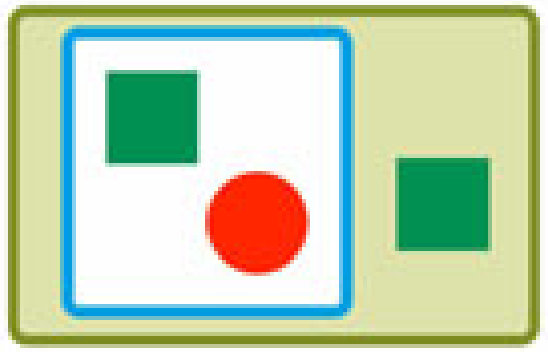
\includegraphics[width=0.06\linewidth]{static/collective2A.png} \ 
\includegraphics[width=0.045\linewidth]{static/collective2B.png}};
    
    
    \node[latent, right=of c2, xshift=1cm] (c1) {$C^1$};
    \node[const, above=of c1, yshift=0.1cm] (pc1) {$P(C^1|C^2)$};
    \node[const, above=of pc1, yshift=0.1cm] (nc1) {Col\en{l}ectiv\en{e}\es{o} 1};
    \node[const, above=of nc1] (fc1) {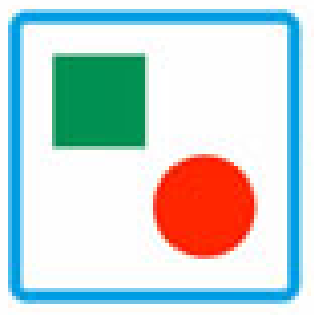
\includegraphics[width=0.04\linewidth]{static/collective1A.png} \ 
\includegraphics[width=0.04\linewidth]{static/collective1B.png}};
    
    \node[latent, right=of c1, xshift=1cm] (i) {$I$};
    \node[const, above=of i, yshift=0.1cm] (pi) {$P(I|C^1,C^2)$};
    \node[const, above=of pi, yshift=0.1cm] (ni) {Individu\en{al}\es{o}:};
    \node[const, above=of ni] (fi) {
\includegraphics[width=0.09\linewidth]{static/individual.png}\ };
    
    \node[latent, right=of i, xshift=1cm] (a) {\en{$e$}\es{$a$}};
    \node[const, above=of a, yshift=0.1cm] (pa) {$P(\en{e}\es{a}|I,C^1,C^2)$};
    \node[const, above=of pa, yshift=0.1cm] (na) {\en{Environment}\es{Ambiente}};
    \node[const, above=of na] (fa) {
\includegraphics[width=0.03\linewidth]{static/water.png}
\includegraphics[width=0.04\linewidth]{static/wind.png}
\includegraphics[width=0.025\linewidth]{static/fire.png} \ };
    
    \edge {c2} {c1};
    \edge {c1} {i};
    \edge {i} {a};
    \path[draw, ->, fill=black,sloped] (c2) edge[bend right,draw=black] node[midway,above,color=black] {} (i);
    \path[draw, ->, fill=black,sloped] (c2) edge[bend right,draw=black] node[midway,above,color=black] {} (a);
    \path[draw, ->, fill=black,sloped] (c1) edge[bend right,draw=black] node[midway,above,color=black] {} (a);
    
    \plate {aa} {(a)} {}; 
    }
\caption{% \en{Model proposed by Czégel, Zachar and Szathmáry~\cite{czegel2019-bayesianEvolution} to represent multilevel selection. }%% \es{Modelo propuesto por Czégel, Zachar y Szathmáry~\cite{czegel2019-bayesianEvolution} para representar selección multinivel. }%
}

\label{fig:czegel_et_el}
\end{figure}
%
La validez de este modelo es trivial en tanto la regla del producto siempre permite la descomposición,
%
\begin{equation}
P(e,I,C^1,C^2)= P(e|I,C^1,C^2)P(I|C^1,C^2)P(C^1|C^2)P(C^2)
\end{equation}
%
Sin embargo el modelo no expresa una interpretación causal.
%
Esto se constata en todas las distribuciones de probabilidad condicional.
%
En un extremo, la colectividad de nivel 2, que está compuesta tanto por la colectividad de nivel 1 y por individuos, aparece en el modelo como una variable independiente.
%
En el otro extremo, el ambiente, que suele considerarse en los modelos causales como una variable aleatoria independiente, aparece en el modelo como dependiente de los individuos y colectividades.
%
Y a la inversa, todas las colectividades e individuos aparecen independientes del ambiente.
%
Esto quizás explique porque en el artículo evitaron especificar las ditribuciones de probabilidad condicional, y ofrecieron en cambio un ejemplo pictórico de la distribución de probabilidad conjunta.

% Parrafo

Interpretemos el modelo de Ole Peters en términos causales para definir las distribuciones de probabilidad condicional.
%
La probabilidad del ambiente, en este caso depende de un parámetro $p$ que determina cuan sesgada está la moneda.
%
\begin{equation}
P(\en{e}\es{a}) = p^{\en{e}\es{a}} (1-p)^{(1-\en{e}\es{a})}
\end{equation}
%
Para definir la probabilidad de las estrategia dado el ambiente, $P(e|a)$, necesitamos que para cada ambiente la probabilidad de todas las estrategias sume 1.
%
Digamos, por ahora, que la probabilidad de la estrategia es proporcional a su aptitud, 
%
\begin{equation}\label{eq:probabilidad_propro_aptitud}
P(\E | \A) \propto  f_{\E}(\A)
\end{equation}
%
Con esto podemos definir parcialmente un modelo gráfico con una interpretación causal.
%
\begin{figure}[H]
\centering
\tikz{
    \node[latent] (e) {$\en{e}\es{a}_t$};
    \node[const, right=of e] (en) {\ $P(\en{e}\es{a}) = p^{\en{e}\es{a}} (1-p)^{(1-\en{e}\es{a})}$};
    \node[const, left=of e] (ne) {\en{Environment}\es{Ambiente}: \ \ \ };
    
    
    \node[latent, below=of e] (r) {$\en{s}\es{a}$};
    \node[const, right=of r] (rn) {$P(\en{s}\es{a}|\en{e}\es{a}) \propto f_e(a)$};
    \node[const, left=of r] (nr) {\en{Strategy}\es{Estrategia}: \ \ \ };
    
    \edge {e} {r};
    \plate {ee} {(e)} {$t$}; 
    }
\caption{Modelo causal Lewontin-Peters}
\label{fig:model-lewontin-peters}
\end{figure}
%
¿Cómo podemos calcular la probabilidad de $P(\E|\A)$?

\subsection{Sum-product algorithm}

\en{The \emph{sum-product algorithm} takes advantage of the factoriztion of the joint probability distribution, induced by the causal model, to efficiently apply the rules of probability. }%
\es{El \emph{sum-product algorithm} aprovecha la factorización de la distribuci\'on de probabilidad conjunta, inducida por el modelo causal, para aplicar eficientemente las reglas de la probabilidad. }%
%
\en{It is a way of computing the rules of probability (the sum and product rule) by message passing between probability distributions and their variables. }%
\es{Es una forma de computar las reglas de la probabilidad (la regla de la suma y el producto) mediante pasaje de mensajes entre las distribuciones de probabilidad y sus variables. }%
%
\en{For this purpose, it is convenient to represent the graphical model with a \emph{factor graph}, a bipartite graph with variable nodes (white circles) and function nodes (black squares). }%
\es{Para ello es conveniente representar el modelo mediante un \emph{factor graph}, un gráfos con nodos variables (círculos blancos), y nodos funciones (cuadrados negros). }%
%
\en{The edge between node variables and node functions represents the mathematical relationship ``the variable $v$ is an argument of the function $f$''. }%
\es{Los ejes entre nodos variables y nodos funciones representan la relaci\'on matem\'atica ``la variable $v$ es argumento de la funci\'on $f$''. }%
%
El siguiente factor graph representa el modelo de la figura \ref{fig:model-lewontin-peters}.
%
\begin{figure}[H]
\centering
\tikz{

    \node[factor] (fa) {};
    \node[const, above=of fa] (nfa) {$P(\A)$};
    
    \node[latent, right=of fa] (a) {$\A$};
    
    \node[factor, right=of a] (fe) {};
    \node[const, above=of fe] (nfe) {$P(\E|\A) \propto f_{\E}(\A)$};
    
    \node[latent, right=of fe, xshift=0.3cm] (e) {$\E$};
    

     \plate {hola} {(fa)(nfa)(a)(fe)(nfe)} {}; 

    \edge[-] {fa} {a};
    \edge[-] {a} {fe};
    \edge[-] {fe} {e};
    }
\caption{
 \en{Graphical way of representing the factorization of joint distribution induced by the basic causal model (Fig.~\ref{fig:model-lewontin-peters}). }%
 \es{Forma gráfica de representar la factorizaci\'on de la distribución conjunta inducida por el modelo causal básico (figura~\ref{fig:model-lewontin-peters}). }%
 }
\label{fig:factor_graph}
\end{figure}
%
\en{There are two types of messages: those sent by variable-type nodes to their function-type neighbors ($m_{v \rightarrow f}(v)$) and the ones that function-type nodes send to their variable-type neighbors ($m_{f \rightarrow v}(v)$). }%
\es{Hay dos tipos de mensajes: los mensajes que envian los nodos variables a sus funciones vecinas ($m_{v \rightarrow f}(v)$); y los mensajes que env\'ian los nodos funciones a sus variables vecinas ($m_{f \rightarrow v}(v)$). }%
%
\en{The former partially performs the product rule. }%
\es{El primero codifica una porci\'on de la regla del producto. }%
%
\begin{equation*}\label{eq:m_v_f} \tag{\text{\en{product step}\es{paso del producto}}}
m_{v \rightarrow f}(v) = \prod_{h}^{n(v) \setminus \{f\} } m_{h \rightarrow v}(v)
\end{equation*}
%
\en{where $n(v) \setminus \{f\}$ represents the set of neighbor nodes to $v$ except $f$. }%
\es{donde $n(v) \setminus \{f\}$ representa el conjunto de vecinos del nodo $v$ salvo $f$. }%
%
\en{In a brief, the messages sent by the variable-type node $v$ are simply the product of the messages that $v$ receives from the rest of their neighbors $h \in n(v)$ except $f$. }%
\es{En pocas palabras, los mensajes que env\'ia una variables $v$ es simplemente la multiplicaci\'on de los mensajes que recibi\'o del resto de sus vecinos $h \in n(v)$ salvo $f$. }%
%
\en{The messages sent by the function-type nodes encode a portion of the sum rule. }%
\es{Los mensajes que env\'ian los nodos funciones codifican una parte de la regla de la suma. }%
%
\begin{equation*}\label{eq:m_f_v}  \tag{\text{\en{sum step}\es{paso de la suma}}}
m_{f \rightarrow v}(v) = \sum_{\bm{u}} \Big( f(\bm{u},v) \prod_{u}^{\bm{u}} m_{u \rightarrow f}(u) \Big)
\end{equation*}
%
\en{where $\bm{u} = n(f)\setminus \{v\}$ is the set of all neighbors to $f$ except $v$, and $f(\bm{h},v)$ represents the function $f$, evaluated in all its arguments. }%
\es{donde $\bm{u} = n(f)\setminus \{v\}$ es el conjunto de todos los vecinos de $f$ salvo $v$, y $f(\bm{h},v)$ representa la funci\'on $f$, evaluada en todos sus argumentos. }%
%
\en{The messages sent by the function-type node $f$ to a neighboring variable-type node $v$ is simply the integration (or sum) over $\bm{h}$ of the product of itself and all the messages that $f$ receives from the rest of its neighbors $\bm{h}$ except $v$. }%
\es{En pocas palabras, los mensajes que envía una funci\'on $f$ a una variable vecina $v$ es simplemente la integraci\'on (o suma) sobre $\bm{h}$ del producto de sí mismo con todos los mensajes que $f$ recibe del resto de sus vecinos $\bm{h}$ salvo $v$. }%
%
\en{Finally, the marginal probability distribution of a variable $v$ is simply the product of the messages that $v$ receives from all its neighbors. }%
\es{Finalmente, la distribuci\'on de probabilidad marginal de una variable $v$ es simplemente la multiplicaci\'on de los mensajes que $v$ recibe de todos sus vecinos. }%
%
\begin{equation*}\label{eq:marginal}  \tag{\text{\en{marginal probability}\es{probabilidad marginal}}}
P(v) = \prod_{h \in n(v)} m_{h \rightarrow v}(v)
\end{equation*}
%
Cuando alguno de las variables $u$ es observable, se la elimina de la suma $\bm{u}\setminus u$ y se obtiene la marginal de dos variables, $P(v,u)$.
%
\en{This algorithm encodes the minimum number of steps required to calculate any marginal probability distribution. }%
\es{Este algoritmo codifica la m\'inima cantidad de pasos que se requieren para calcular cualquier distribuci\'on de probabilidad marginal. }%

% Parrafo

Nosotros queremos calcular $P(\E|\A)$ y para eso necesitamos calcular marginales $P(\E,\A)/P(\A)$. 
%
Como en nuestro modelo una de las distribuciones de probabilidad está definida de forma proporcional, las marginales $P(\E,\A)$ y $P(\A)$ también serán proporcionales.
%
Para calcular la marginal $P(\E,\A)$, consideraremos que $\A^*$ es observable.
%
El mensaje del factor del ambiente $f_{\A}$ a la variable ambiente $\A$ es,
\begin{equation}
m_{f_{\A}\rightarrow \A }(\A^*) = P(\A^*) = m_{f_{\A} \rightarrow f_{\E} }(\A^*)
\end{equation}
%
Que es el mismo mensaje que envía la variable $\A$ al factor de estrategias $f_{\E}$.
%
Luego, el mensaje que envía el factor de estategias $f_{\E}$ a la variable estrategias es,
%
\begin{equation}
m_{f_{\E} \rightarrow \E } \propto P(\A^*)f_{\E}(\A)
\end{equation}
%
Notar que no integramos en los valores del ambiente porque consideramos que la variable $\A$ es observable.
%
Luego, la marginal de un vector de observaciones del ambiente $\bm{\A}$ es,
%
\begin{equation}
P(\E,\bm{\A}) \propto \prod_{\A^*}^{\bm{\A}} P(\A^*)f_{\E}(\A^*)
\end{equation}
%
Integrando sobre las estrtategia $\E$ obtenemos la marginal de las observaciones,
%
\begin{align}
P(\bm{\A}) & \propto \sum_{\E} \prod_{\A^*}^{\bm{\A}} P(\A^*)f_{\E}(\A^*) \\
& = \prod_{\A^*}^{\bm{\A}} P(\A^*)  \sum_{\E} \prod_{\A^*}^{\bm{\A}}f_{\E}(\A^*)
\end{align}
%
Luego, la probabilidad de la estrategia dado el ambiente es
%
\begin{equation}\label{eq:replicator_dynamic_posterior}
P(\E|\bm{\A}) = \frac{ \prod_{\A^*}^{\bm{\A}}f_{\E}(\A^*)}{\sum_{\E} \prod_{\A^*}^{\bm{\A}}f_{\E}(\A^*)}
\end{equation}
%
La probabilidad condicional de la estrategia dado el ambiente resultó ser el replicator dynamic!
%
Es decir, el replicator dynamic surgió de considerar el modelo causal en el que el ambiente causa las estretgias y en el que las el tamaño de las estrategias depende de la adaptabilidad de esa estrategia al ambiente.

% Parrafo

El ejemplo Lewontin-Peters considera una única estrategia.
%
Nuestro modelo permite elegir el conjunto de estrategias que queramos.
%
Si bien podemos proponer cualquier tipo de estrategia, vamos a limitarnos a aquellas que tienen un recurso $R$ para repartir entre cara y sello.
%
\begin{equation}
f_{\E}(\A) = \begin{cases}
 \E & \A = 1 \\
 R-\E & \A = 0
  \end{cases}
\end{equation}
%
con $ 0 \leq \E \leq R$.
%
Esta familia de funciones de apritud son proporcionales a la distribución de probabilidad Bernoulli.
%
\begin{equation}
\text{P}(\E|\A) = \E^\A \cdot (1-\E)^{(1-\A)} = \text{Bernoulli}(\E|\A)
\end{equation}
%
con $ 0 \leq \E \leq 1$.
%
La estrategia $\E \approx 0.71$ es la propuesta por Ole Peters, y la la estraetgia $\E \approx 0.77$ es la propuesta por Lewontin y Cohen.
%
Cuando consideramos las ifnitias estraetgias que tienen un recurso $R$ fijo, el posterior de la estretgia $\E$ dado un vector de observaciones del ambiente $\bm{a}$ tiene solución analítica y pertenecerá a la distribución Beta (notar que el denominador de la ecuación \ref{eq:replicator_dynamic_posterior} es la función Beta o la integral de Euler).
%
\begin{equation}
P(\E|\bm{\A}) = \text{Beta}(\texttt{sum}(\bm{\A}), \, \texttt{length}(\bm{\A}) - \texttt{sum}(\bm{\A}))
\end{equation}
%
Este modelo nos permitirá analizar la estabilidad evolutiva del espacio de estrategias desertoras. 
Supongamos que la moneda está sesgada de modo que el $0.71$ de las veces sale cara y el $0.29$ sale seca.
En las siguientes figuras mostramos cómo cambia la proporción de las estrategias a medida que agregamos observaciones al modelo.
%
\begin{figure}[H]
    \centering
    \begin{subfigure}[b]{0.32\textwidth}
    \includegraphics[width=\linewidth]{figures/coin1.pdf}
    \caption{$T = 1$}
    \end{subfigure}
    \begin{subfigure}[b]{0.32\textwidth}
    \includegraphics[width=\linewidth]{figures/coin2.pdf}
    \caption{$T = 10$}
    \end{subfigure}
    \begin{subfigure}[b]{0.32\textwidth}
    \includegraphics[width=\linewidth]{figures/coin3.pdf}
    \caption{$T = 10^5$}
    \end{subfigure}
    \caption{Densidad (eje y) de las diferentes estrategias desertoras (eje x) a medida que avanza el juego ($T=1, \, T=10, \, T=10^5$).}
    \label{fig:estrategias_individuales}
\end{figure}
%
El proceso evolutivo selecciona las estrategias individuales que reparten los recursos en la misma proporción que se generan los estados del ambiente.
Cuando el ambientes genera los estados con una probabilidad de $p*=0.71$, entonces la estrategia individual mejor adaptada es la que en cada ronda apuesta $0.71$ de sus recursos al ambiente $a=1$, y $0.29$ de sus recursos al ambiente $a=0$.

% Parrafo

El ejemplo de Ole Peters supone que la moneda no está sesgada.
En este contexto, la estrategia utilizada por él para mostrar la ventaja de la cooperación no es la que está mejor adaptada en términos individuales.
¿Las estrategias individuales que mejor se adaptaron al ambiente tienen la misma tasa de crecimiento temporal que la de los grupos cooperativos?
¿Que ocurre cuando la probabilidad del ambiente estocástico varía? 
¿Será que si la probabilidad del ambiente no cambia, no hay ninguna ventaja a favor de la cooperación?
Responderemos estas y otras preguntas en la siguiente sección.
%Si ese fuera el caso, un pequeño costo asociado a la coordinación haría generaría una ventaja a favor de las estrategias individuales.
%Al menos en ambientes estocásticos estables, que mantinen 

\section{Resultados}


En esta sección analizaremos si efectivamente existe alguna ventaja evolutiva de la cooperación y la especialización en presencia de deserción.
Para ello analizaremos la selección multinivel medainte modelos causales probabilísiticos.


\subsection{Modelo multinivel}

Supongamos que tenemos grupos de $N$ individuos en el que $n$ son cooperadores y $N-n$ desertores.
%
Con $N$ individuos, hay $N+1$ tipos de grupos posibles, desde $n=0$ (todos desertores) hasta $n=N$ (todos cooperadores).
%
Luego, si cada individuo pertenece a un único grupo necesitamos $M = N(N+1)$ individuos totales, $i \in \{1, \dots, M\}$.
%
Los individuos están caracterizados por tres atributos: el vector de estrategias $\bm{\Ee} = (\Ee_1, \dots, \Ee_M)$, que es un parámetro del modelo (en el caso más simple, todos los individuos tienen la misma estrategia); el grupo al que pertenecen, $\texttt{grupo}(i) = i \ \texttt{div} \ N$, definido como la división entera por $N$; y el comportamiento social, $\texttt{coop}(i) = i \ \texttt{mod} \ N < \texttt{grupo}(i)$, los primeros $n$ individuos del grupo son cooperadores y el resto desertores.
%
Como antes, el ambiente $\A$ es una variable independiente que con probabilidad $p$ sale cara y con probabilidad $1-p$ sale sello, $P(\Aa) = p^\Aa (1-p)^{1-\Aa}$, pero ahora en cada tiempo $t$ tenemos un vector $\bm{\Aa}$, en el que cada elemento influencia al $i-$ésimo agente, $P(i|\bm{\Aa}) = \bm{\Ee}_i^{\bm{\Aa}_i} (1-\bm{\Ee}_i)^{\bm{\Aa}_i$.
%
Ahora sin embargo, los agentes también están influenciados por los recursos del los otros agentes en el tiempo anterior, 
%
\begin{equation}
P(i^{t+1}|i^t) = 
\begin{cases}
1/N & \texttt{coop}(i^t) \text{ y } (\texttt{grupo}(i^{t+1}) = \texttt{grupo}(i^{t})) \\
1 & \neg \texttt{coop}(i^t) \text{ y } i^{t+1} = i^t \\
0 & \texttt{else} \\
\end{cases}
\end{equation}
%
Los individuos cooperadores dividen la riqueza en partes iguales con los miembros de su grupo, y los individuos desertores se quedan con toda su riqueza.
%
Finalmente, los grupos dependen de los individuos que los integran $P(g|i)=\mathbb{I}(\texttt{grupo}(i) = g)$, la función indiciadora que vale $1$ para los individuos que forman parte del grupo $g$ y $0$ para el resto.
%
\begin{figure}[H]
\centering
 \begin{subfigure}[b]{0.4\textwidth}    
 \centering
 \tikz{
    
    \node[obs] (a1) {$\vec{\A}^{\,1}$};
    \node[obs, right=of a1] (a2) {$\vec{\A}^{\,2}$};
    
    \node[latent, below=of a1 ] (i1) {$I^1$};
    \node[latent, below=of a2 ] (i2) {$I^2$};
    \node[latent, right=of i2 ] (i3) {$I^3$};

    \node[latent, below=of i1 ] (c1) {$G^1$};
    \node[latent, below=of i2 ] (c2) {$G^2$};
    \node[latent , below=of i3 ] (c3) {$G^3$};
    
    \node[invisible, below=of c2, yshift=-0.5cm] (inv) {};
    
    
    \edge {a1} {i1};
    \edge {a2} {i2};
    \edge {i1} {i2,c1};
    \edge {i2} {i3,c2};
    \edge {i3} {c3};
    
    }
 \caption{Red bayesiana}
 \label{fig:red_bayesiana_multinivel}
 \end{subfigure}
\begin{subfigure}[b]{0.58\textwidth}    
 \centering
 \tikz{
    
    \node[factor] (fa1) {};
    \node[obs, yshift=0.5cm, below=of fa1] (a1) {$\vec{\A}^{\,1}$};
    
    \node[factor, yshift=0.5cm, below=of a1] (fia1) {};
    
    \node[latent, yshift=0.5cm, below=of fia1 ] (i1) {$I^1$};
    
    \node[factor, xshift=-0.3cm, right=of i1] (fii1) {};
    \node[factor, yshift=0.5cm, below=of i1] (fg1) {};
    \node[latent, yshift=0.5cm, below=of fg1 ] (g1) {$G^1$};
    
    \node[latent, xshift=-0.3cm, right=of fii1 ] (i2) {$I^2$};
    
    \node[factor, yshift=-0.5cm, above=of i2] (fia2) {};
    \node[obs, yshift=-0.5cm, above=of fia2] (a2) {$\vec{\A}^{\,1}$};
    \node[factor, yshift=-0.5cm, above=of a2] (fa2) {};
    \node[factor, yshift=0.5cm, below=of i2] (fg2) {};
    \node[latent, yshift=0.5cm, below=of fg2 ] (g2) {$G^2$};
    
    \node[factor, xshift=-0.3cm, right=of i2] (fii2) {};
    
    \node[latent, xshift=-0.3cm, right=of fii2 ] (i3) {$I^3$};
    \node[factor, yshift=0.5cm, below=of i3] (fg3) {};
    \node[latent, yshift=0.5cm, below=of fg3 ] (g3) {$G^3$};
    
     \node[const, left=of fa1] (pa) {$P(\bm{\Aa})$};
     \node[const, left=of fia1] (pea) {$P(i|\bm{\Aa})$};
     \node[const, left=of fg1] (pg) {$P(g|i)$};
     \node[const, above=of fii2] (pee) {$P(i^{t+1}|i^t)$};
     
    \edge[-] {a1} {fa1, fia1};
    \edge[-] {a2} {fa2, fia2};
    \edge[-] {i1} {fii1,fg1,fia1};
    \edge[-] {i2} {fii1, fii2,fg2,fia2};
    \edge[-] {i3} {fii2, fg3};
    \edge[-] {g1} {fg1};
    \edge[-] {g2} {fg2};
    \edge[-] {g3} {fg3};
    }
 \caption{Factor graph}
 \label{fig:factor_graph_multinivel}
 \end{subfigure}
\caption{Modelo multinivel. Figura~\ref{fig:red_bayesiana_multinivel}: la red de dependencias probabilísiticas que surge del modelo causal multinivel. Figura~\ref{fig:factor_graph_multinivel}: el grafo de factores inducido por la red bayesiana, que será utilizado para aplicar el algoritmo suma-producto. Las variables pintadas de gris se consideran observables. }
\label{fig:multilevel_model}
\end{figure}
%
En resumen, en cada tiempo $t$ el ambiente influencia a los individuos, y los individuos influencian a los grupos de su propio tiempo y a los individuos del tiempo $t+1$.
%
Este modelo tiene $3$ hiperparámetros: el vector de estrategias $\bm{\Ee}$, la probabilidad del ambiente $p$, y el tamaño de los grupos $N$.
%
Este modelo se puede simplificar levemente, usando una única variable de grupo que dependa de la última variable individuo, gracias a que la margnial de los grupos es la misma en cualquier tiempo $t$.

% Parrafo

En el problema evolutivo nos va a interesar la selección de los individuos cooperadores dado el ambiente dentro de cada grupo (nivel 1), $P(\texttt{coop}(i^T)|\bm{\Aa}^1, \dots, \bm{\Aa}^{T-1}, g)$, la selección de los grupos dado el ambiente (nivel 2), $P(g^T|\bm{\Aa}^1, \dots, \bm{\Aa}^{T-1})$, y la selección de los individuos cooperadores dado el ambiente integrando todos los grupos (multinivel), $P(\texttt{coop}(i^T)|\bm{\Aa}^1, \dots, \bm{\Aa}^{T-1})$.
%
% \begin{table}[H]
% \centering
% \begin{tabular}{ccc}
%         Selección de nivel 1 & Selección de nivel 2 & Selección multinivel\\ 
%         $P(\texttt{coop}(i^T)|\bm{\Aa}^1, \dots, \bm{\Aa}^{T-1}, g)$ & $P(g^T|\bm{\Aa}^1, \dots, \bm{\Aa}^{T-1})$ & $P(\texttt{coop}(i^T)|\bm{\Aa}^1, \dots, \bm{\Aa}^{T-1})$ \\ 
% \end{tabular}
% \end{table}
%
La selección multinivel se obtiene integrando el producto de las selecciones de nivel 1 y 2, 
%
\begin{equation}\label{eq:posterior_multinivel}
\underbrace{P(\texttt{coop}(i^T)|\bm{\Aa}^1, \dots, \bm{\Aa}^{T-1})}_{\text{Selección multinivel}} = \sum_{g=0}^N \underbrace{P(\texttt{coop}(i^T)|\bm{\Aa}^1, \dots, \bm{\Aa}^{T-1}, g)}_{\text{Selección de nivel 1}} \cdot \underbrace{P(g^T|\bm{\Aa}^1, \dots, \bm{\Aa}^{T-1})}_{\text{Selección de nivel 2}}
\end{equation}
%
donde el posterior de la selección de nivel 1 se obtiene integrando la probabilidad de todos los individuos cooperadores que forman parte del grupo $g$,
%
\begin{equation}\label{eq:posterior_nivel_1}
\begin{split}
P(\texttt{coop}(i^T)|\bm{\Aa}^1, \dots, \bm{\Aa}^{T-1}, g) &= \sum_{j=1}^M P(I^T=j|\bm{\Aa}^1, \dots, \bm{\Aa}^{T-1}, g)\mathbb{I}(\texttt{coop}(j) \text{ y } \texttt{grupo}(j)=g)
\end{split}
\end{equation}

% Parrafo

Para calcular los posteriors va a ser suficiente con calcular las probabilidades marginales, pues ambas expresiones son proporcionales.
%
Las probabilidades marginales se pueden obtener mediante el sum-product algorithm en un modelo como el de la figura~\ref{fig:multilevel_model} pero que tiene como observables las variables que en el posterior aparecen en el condicional.
%
Ya hemos visto en la sección metodología que la probabilidad marginal de una variable $v$ es el producto de los mensajes que recibe de los nodos vecinos del factor graph.
%
Las variables observables no deben integrarse cuando se aplica el sum-product algorithm, por lo que la marginal de $v$ será la probabilidad conjunta de $v$ y todas las variables observables del modelo.
%
La probabilidad marginal de los individuos en el tiempo $T$ cuando tenemos como observable todos los ambientes $\bm{\Aa}^{t}$ y el grupo $g$ es, 
%
\begin{equation}\label{eq:posterior_individuos_dado_grupo}
P(i^{T},\bm{\Aa}^1, \dots, \bm{\Aa}^{T-1}, g) = m_{P(i^{T}|i^{T-1}) \rightarrow i^T}(i^T) \cdot m_{P(g^{T}|i^{T}) \rightarrow i^T}(i^T) 
\end{equation}
%
el producto de los mensaje que la variable $i^T$ recibe del factor social $P(i^{T}|i^{T-1})$ y del factor de grupo $P(g^{T}|i^{T})$, en el modelo que tiene al conjunto $\{ \bm{\Aa}^1, \dots, \bm{\Aa}^{T-1}, g\}$ como variables observables.
%
La probabilidad marginal de los grupos en el tiempo $T$, cuando tenemos como observable todos los ambientes $\bm{\Aa}^{t}$ es, 
%
\begin{equation}\label{eq:posterior_nivel_2}
P(g^{T},\bm{\Aa}^1, \dots, \bm{\Aa}^{T-1}) = m_{P(g^{T}|i^{T}) \rightarrow g^T}(g^T)
\end{equation}
%
el mensaje que la variable $g^T$ recibe del factor de grupo $P(g^{T}|i^{T})$, en el modelo que tiene a $\{ \bm{\Aa}^1, \dots, \bm{\Aa}^{T-1}\}$ como observables.
%
Una forma alternativa de calcular la marginal de los selección multinivel (Eq.~\ref{eq:posterior_multinivel}) es integrando la probabilidad de los individuos cooperadores dado los ambientes
\begin{equation}\label{eq:posterior_multinivel_alternativa}
\begin{split}
P(\texttt{coop}(i^T)|\bm{\Aa}^1, \dots, \bm{\Aa}^{T-1}) &= \sum_{j=1}^M P(I^T=j|\bm{\Aa}^1, \dots, \bm{\Aa}^{T-1})\mathbb{I}(\texttt{coop}(j))
\end{split}
\end{equation}
%
donde la probabilidad de los individuos cuando tenemos como observable todos los ambientes $\bm{\Aa}^{t}$ es,
%
\begin{equation}
P(i^{T},\bm{\Aa}^1, \dots, \bm{\Aa}^{T-1}) = m_{P(i^{T}|i^{T-1}) \rightarrow i^T}(i^T)
\end{equation}
%
el mensaje que la variable $i^T$ recibe del factor de social $P(i^{T}|i^{T-1})$ en el modelo que tiene a $\{ \bm{\Aa}^1, \dots, \bm{\Aa}^{T-1}\}$ como observables.
%
En resumen, necesitamos calcular solamente tres mensajes.
%
\begin{table}[H]
\centering
\begin{tabular}{cccc}
 Mensajes & $m_{P(g^{T}|i^{T}) \rightarrow i^T}(i^T)$ & $m_{P(g^{T}|i^{T}) \rightarrow g^T}(g^T)$ & $m_{P(i^{T}|i^{T-1}) \rightarrow i^T}(i^T)$ \\[0.1cm]
 Observables & $\{g\}$ &  $\{ \bm{\Aa}^1, \dots, \bm{\Aa}^{T-1}\}$ &   $\{ \bm{\Aa}^1, \dots, \bm{\Aa}^{T-1}\}$\\ 
 & & & 
\end{tabular}
\caption{Los mensajes que componen las marginales de la selección de nivel 1, 2 y multinivel.}
\end{table}
%
El primer mensaje, que envía el factor de grupo a la variable individuo cuando la variable de grupo es observable, es
\begin{equation}
 m_{P(g^{T}|i^{T}) \rightarrow i^T}(i^T) = P(g|i) = \mathbb{I}(\texttt{grupo}(i) = g)
\end{equation}
%
la función indiciadora que vale $1$ para los individuos que forman parte del grupo $g$ y $0$ para el resto.
%
El segundo mensaje, que el factor grupo envía a la variable grupo, es
%
\begin{equation}
 m_{P(g^{T}|i^{T}) \rightarrow g^T}(g^T) = \sum_i P(g|i) m_{P(i^{T}|i^{T-1}) \rightarrow i^T}(i^T) 
\end{equation}
%
el cual está compuesto por el tercer mensaje, que el factor social envía a la variable individuo.
%
Para computar este tercer y último mensaje debemos calcular los mensajes precedentes que lo componen.
%
Entre ellos están los mensajes que el factor ambiente envía a la variable ambiente,
%
\begin{equation}
m_{P(\vec{\Aa}^{\,t})\rightarrow \vec{\Aa}^{\,t}}(\vec{\Aa}^{\,t}) = P(\vec{\Aa}^{\,t}) = m_{\vec{\Aa}^{\,t} \rightarrow P(i^t|\vec{\Aa}^{\,t})} (\vec{\Aa}^{\,t})
\end{equation}
%
que es el mismo mensaje que la variable ambiente envía al factor individuo.
%
Luego podemos generar el mensaje que envía el factor individuo a la variable individuo, 
%
\begin{equation}
m_{P(i^t|\vec{\Aa}^{\,t}) \rightarrow i^t}(i^t) = P(\vec{\Aa}^{\,t}) \, P(i^t|\vec{\Aa}^{\,t})
\end{equation}
%
que como la variable ambiente es observable, no incluye la integración que suelen hacer los mensajes que envían los factores.
%
Y por último, el mensaje que la variable individuo envía al factor social,
%
\begin{equation}\label{eq:m_i_pii}
\begin{split}
m_{i^t \rightarrow P(i^{t+1}|i^t)}(i^t) =m_{P(i^t|\vec{\Aa}^{\,t}) \rightarrow i^t}(i^t) m_{P(i^t|i^{t-1}) \rightarrow i^t }(i^t) & = P(\vec{\Aa}^{\,t}) \, P(i^t|\vec{\Aa}^{\,t}) \text{Prior}(i^t)
\end{split}
\end{equation}
%
donde $\text{Prior}(i^t) = m_{P(i^t|i^{t-1}) \rightarrow i^t }(i^t)$ es el mensaje que la variable individuo recibe del factor social pasado.
%
No incluimos en la multiplicación el mensaje que el factor de grupo envía a la variable individuo porque al no ser observable se cancela automáticamente, $m_{P(g^t|i^{t}) \rightarrow i^t}(i^t) = \sum_g P(g|i^t) = 1$.
%
Notar que la ecuación~\ref{eq:m_i_pii} es proprocional al proceso multiplicativo estudiado por Ole Peters (segundos nodos de la figura \ref{fig:protocolo}), en el que los recursos previos $\omega_i(t)$ se actualizan en función de la aptitud al ambiente $f(\Aa)$.
%
\begin{equation}
\begin{split}
m_{i^t \rightarrow P(i^{t+1}|i^t)}(i^t) & \propto P(i^t|\vec{\Aa}^{\,t}) \text{Prior}(i^t) \propto f_{\Ee_i}(\Aa_{i}^{t}) \text{Prior}(i^t) = f_{\Ee_i}(\Aa_{i}^{t}) \omega_i(t) 
\end{split}
\end{equation}
%
donde el segundo proporcional vale por construcción de la distribución de probabilidad $ P(i^t|\vec{\Aa}^{\,t})$ (ver ecuación~\ref{eq:probabilidad_propro_aptitud}), y donde la igualdad final vale por renombre $\text{Prior}(i^t) = \omega_i(t)$.
%
Finalmente, el tercer mensaje objetivo (que codifica la selección multinivel) introduce el factor social sobre los recursos individuales.
%
\begin{equation}\label{eq:m_pii_i}
\begin{split}
m_{P(i^{t+1}|i^{t}) \rightarrow i^{t+1} }(i^{t+1}) & = \sum_{i^t} P(i^{t+1}|i^t) \, P(\vec{\Aa}^{\,t}) \, P(i^t|\vec{\Aa}^{\,t}) \,  m_{P(i^t|i^{t-1}) \rightarrow i^t }(i^t) 
\end{split}
\end{equation}
%
Este mensaje está definido recursivamente.
%
Para calcularlo lo resolveremos por casos debido a que el factor social es diferente según la población sea enteramente desertora, enteramente cooperadora o mixta.
%
Notar que la ecuación~\ref{eq:m_pii_i} es proprocional a los recursos individuales luego de la redistribución del fondo común,
%
\begin{equation}
\begin{split}
m_{P(i^{t+1}|i^{t}) \rightarrow i^{t+1} }(i^{t+1}) & \propto \sum_{i^t} P(i^{t+1}|i^t) \, P(i^t|\vec{\Aa}^{\,t}) \,  \text{Prior}(i^t) \\
& \propto \sum_{i^t} P(i^{t+1}|i^t) \, f_{\Ee_i}(\Aa_{i}^{t}) \omega_i(t)  = \omega_i(t+1)
\end{split}
\end{equation}
%
Este mensaje generaliza el último nodo de la figura~\ref{fig:protocolo}.

% Parrafo

En la introducción hemos derivado la tasa de crecimiento de esta marginal para los grupos enteramente desertoras y solo hemos presentado un resultado numérico para el grupo enteramente cooperador.
%
En la siguiente sección resolveremos analíticamente la marginal para grupos enteramente cooperadoras y mixtos, y verificaremos la hipótesis de Ole Peters de la ventaja evolutiva de la cooperación.
%
Y la sección \ref{sec:especialization}, haremos uso de los resultado análitico para demostrar la ventaja evolutiva de la especilización, rechazando la hipótesis de Ole Peters de que la especialización es un mecanismo implausible para poblaciones chicas.


\subsection{Selección de nivel 1, nivel 2 y multinivel}

En esta subsección resolveremos la marginal que necesitamos para computar el posterior de la la selección de nivel 1, de nivel 2 y multinivel,
%
\begin{equation}
\begin{split}
P(i^{T+1}, \vec{\Aa}^{\,1}, \dots, \vec{\Aa}^{\,T}) & = m_{P(i^{T+1}|i^{T}) \rightarrow i^{T+1} }(i^{T+1})
\end{split}
\end{equation}
%
donde el mensaje está definido recursivamente en la ecuación~\ref{eq:m_pii_i}.
%
En el anexo lo resolvemos por casos mediante inducción matemática: primero para los individuos del grupo enteramente desertores, luego para los del grupos enteramente cooperadores, y finalmente para los del grupos mixtos.
%
\begin{equation}
P(i^{T+1}, \bm{\Aa}^1, \dots, \bm{\Aa}^T) = 
\begin{cases}
\prod_{t=1}^{T}  P(\vec{\Aa}^{\,t}) P(i^{T+1}|\vec{\Aa}^{\,t}) & \texttt{grupo}(i^{T+1})=0
\prod_{t=1}^{T}  P(\vec{\Aa}^{\,t})  \sum_j^{\texttt{G}(i^{T+1})} \frac{1}{N} P(j|\vec{\Aa}^{\,t}) & \texttt{grupo}(i^{T+1}) = N  \\
 & \texttt{coop}(i^{T+1}) \text{ y } \texttt{grupo}(i^{T+1}) \neq 0 \text{ y } \texttt{grupo}(i^{T+1}) \neq N
\end{cases}
\end{equation}






Posteriors.



\begin{equation}
 P(k|\vec{\Aa}^{\,1},\dots,\vec{\Aa}^{\,T}) = \prod_{t=1}^{T}   \frac{1}{N} \sum_j^{\texttt{socios}(r)} P(j|\vec{\Aa}^{\,t}) 
\end{equation}


\begin{equation}
P(k|\vec{\Aa}^{\,1}, \dots, \vec{\Aa}^{\,T}) = \Big(\prod_{t=1}^{T} P(k|\vec{\Aa}^{\,t}) \Big) + \Big(\sum_{t=1}^{T} P(c|\wedge_{q=1}^t\vec{\Aa}^{\,q})  \prod_{q=t+1}^T P(k|\vec{\Aa}^{\,q}) \Big)
\end{equation}







































\newpage



\subsection{Ventaja evolutiva de la cooperación}

Notar la diferencia entre esta ecuación, y la de ecuación~\ref{eq:marginal_multinivel_desertor}.
%
Los individuos de los grupos enteramente cooperadores juegan con una variable aleatoria, $s_C(\vec{\Aa}\,)$, distinta a la variable aleatoria de la que dependen los individuos de los grupos enteramente desertores.
%
Los posibles fitness cooperativos para la población de tamaño 3 son,
%
\begin{equation}
s_C(\vec{\Aa}\,) =
\begin{cases}
(1-\Ee) & \text{ si } \texttt{sum}(\vec{\Aa}\,) = 0 \\
\frac{1}{3} \Ee + \frac{2}{3} (1-\Ee)  & \text{ si } \texttt{sum}(\vec{\Aa}\,) = 1 \\
\frac{2}{3} \Ee + \frac{1}{3} (1-\Ee)    & \text{ si } \texttt{sum}(\vec{\Aa}\,) = 2 \\
\Ee & \text{ si } \texttt{sum}(\vec{\Aa}\,) = 3
\end{cases}
\end{equation}
%
Y en general, 
\begin{equation}\label{eq:fitness_cooperador}
s_C(\vec{\Aa}\,) = \frac{a}{n} e + \frac{n-a}{n}(1-e)
\end{equation}
%
El fitness conjunto, luego de observar $T$ estados del ambiente, es
%
\begin{equation}
f(\bm{a}|e,n,c=1) = \prod^T_t f(a^t|e,n,c=1)
\end{equation}
%
Donde $\bm{a}$ es el vector de tamaño $T$ con la cantidad de éxitos obtenidos en cada caso.
La tasa de crecimiento característica de los agentes cooperadores la podemos calcular utilizando la media geomética~\ref{eq:geometric_mean},
%
\begin{equation}
\overline{f}(e,n,c=1) = \prod_{a=0}^n f(a|e,n,c=1)^{\text{Binomial}(a|n,p^*)}
\end{equation}
%
donde $p^*$ es la verdadera probabilidad de generación de los estados $a$.
Cuando la población es muy grande, $n\rightarrow \infty$, en cada ronda habrá invariantemente una proproción $p*$ que obtuvo éxito, por lo que el likelihood caracterísitico se reduce a,
%
\begin{equation}
\lim_{n\rightarrow \infty} \overline{f}(e,c=1) = p^* e + (1-p^*)(1-e)
\end{equation}
%
El likelihood temporal caracterísitico de una estrategia $e$ en una población cooperativa infinita es la esperanza, la cual es lineal respecto de la verdadera probabilidad de generación de los estados del ambiente.

%En el siguiente modelo hacemos explícito el tipo de comportamiento $c\in\{0,1\}$ del agente.
%La extensión del modelo de Ole Peters que realizamos en la sección Metodología (figura~\ref{fig:modelo_beta_binomial}) sólo analizamos el comportamiento desertor individual.

\subsection{La ventaja de la especialización}

Conociendo al tasa de crecimiento caracterísitica de la población cooperadora y desertora, podemos analizar qué ocurre con las diferentes estrategias en diferentes ambientes.
En la siguiente figura graficamos el likelihood característico individual (líneas continuas) y cooperativos (líneas punteadas) de tres estrategias ($e \in \{0.5, 0.75, 0.99\}$) para diferentes probabilidades de generación del ambiente.
%
\begin{figure}[H]
    \centering
    \begin{subfigure}[b]{0.66\textwidth}
    \includegraphics[width=\linewidth]{figures/pdf/tasa-temporal-0.pdf}
    \end{subfigure}
    \caption{Likelihood característico bajo regímenes individuales (líneas continuas) y cooperativos infinitos (líneas punteadas) de tres estrategias ($e \in \{0.5, 0.75, 0.99\}$) en diferentes tipos de ambiente $p^*$.}
    \label{fig:fitness_temporal}
\end{figure}
%
La flecha representa la conclusión de Ole Peters que presentamos en la introducción, donde mostramos experimentalmente que en un ambiente que genera los estados con una probabilidad de $p^* = 0.5$, la estretgia $e=0.71$ pasa de una tasa de crecimiento individual equivalente a la media geométrica a una tasa de crecimiento cooperativa equialente a su media aritmética.
El punto rojo representa la conclusión que sacamos en la sección metodología, que en un ambiente con $p^*=0.71$ la estrategia individual mejor adaptada es $e=0.71$.

% Parrafo

Con esta imagen podemos sacar algunas conclusiones nuevas.
Arriba del punto rojo se encuentra el likelihood caracterísitica de la población cooperativa de la estrategia especialista $e=0.99$.

\begin{conclution}[La ventaja de la especialización]
La cooperación ofrece una ventaja a favor de las estrategias especialistas. Estrategias que individualmente están mal adaptadas al ambiente, cooperando superan incluso a la población cooperativa que individualmemte está bien adaptada.
\end{conclution}

Esta conclusión la hemos obtenido a partir de tasa de crecimiento caracterísitica de una población cooperativa infinita.
Para que sea una conclusión interesante este comportamiento debería ocurrir en poblaciones finitas, particularmente pequeñas.
En la siguiente figura graficamos las tasas de crecimiento caracterísitica de la estrategia especialista $e=0.99$ para poblaciones cooperativas de tamaño 1 a 5.
%
\begin{figure}[H]
    \centering
    \begin{subfigure}[b]{0.66\textwidth}
    \includegraphics[width=\linewidth]{figures/pdf/tasa-temporal-1.pdf}
    \end{subfigure}
    \caption{
    Tasa de superviencia temporal de la estrategia especialista ($e=0.99$) en función del ambiente, para diferentes tamaños de población cooperativa (de 1 a 5).
    La línea punteada negra represeta la tasa de crecimiento de una población cooperativa inifinitamente grande.
    Las rectas grises se dejan como referencia visual de las estrtegias $e \in \{0.5, 0.71\}$ analizadas en la figura anterior.
    }
    \label{fig:multilevel-selection-1}
\end{figure}
%
Un población de tres agentes es suficiente para que la estrategia especialista mal adaptada individualmente, logre cooperativamente superar a la población cooperativa compuesta de estrategia individualmente bien adapatadas!
Es realmente extraordinario que un sistema tan simple como el que estamos analizando tenga conclusiones tan fudamentales para entender la complejidad de la vida.
El proceso multiplicativo al cuál está sujeto la vida favorece tanto la cooperación como la especialización.

% Parrafo

El nivel de especialización depende del tamaño de la población.
Para analizarlo, fijamos el ambiente en $p^* = 0.71$ y analizamos como varía la tasa de crecimiento caracterísitica cooperativa para todo el rango de estrategias para diferentes tamaños de población (de 1 a 5).
%
\begin{figure}[H]
    \centering
    \begin{subfigure}[b]{0.66\textwidth}
    \includegraphics[width=\linewidth]{figures/pdf/tasa-temporal-2.pdf}
    \end{subfigure}
    \caption{
    La tasa de crecimiento temporal de las estretgias para diferentes tamaño de población enteramente cooperativa (de 1 a 5) en un ambiente $p^*=0.71$.
    }
    \label{fig:multilevel-selection-1}
\end{figure}
%
Ele eje x representa las diferentes estrategias.
Cada una de las curvas representa un tamaño de población cooperativa.
Los puntos indican la estretgia óptima para el tamaño de la población.
Cuando la población tiene tamaño 1, la estrategia mejor adaptada es la que apuesta con la misma probjabilidad que el ambiente.
Pero rápidamente, a medida que aumentamos el tamaño de la población, la cooperación favorece a las estrategias especialistas hasta que en poblaciones de tamaño inifinto el nivel se alcanza un nivel de especialización total que logra la tasa de crecimiento máxima, que es equivalente a la probabilidad de generación de las aptitudes $p^*$.

\subsection{Selección multinivel}

Para concluir que existe una ventaja evolutiva a favor de la cooperación y la especialización hace falta demostrar que la cooperación, no sólo puede resisitir la invasión de mutantes desertores, sino que ella misma invadirá poblaciones de desertores una vez que aparece.
Para empezar, veamos qué ocurre en poblaciones de tamaño 2.

% 

En la introducción hemos visto que, si bien la deserción unilateral produce pérdidas en términos absolutos para el mismo agente desertor sin necesidad de introducir castigos, los mutantes desertores invadirán evolutivamente la población debido a que su tasa de crecimiento será mayor que la del agente cooperador.
¿Pero qué ocurre con las diferentes tipos de poblaciones?
Una vez que surge una población enteramente cooperadora, ¿ésta es capaz de invadir el resto de poblaciones no cooperadoras?.

% Parrafo

Para responder esta pregunta extenderemos el modelo bayesiano, incluyendo un nuevo nivel superior: el tipo de grupo.
En una población de tamaño 2 tenemos 4 configuraciones posibles: CC, CD, DC, DD.
Definiendo un prior uniforme sobre estas 4 configuraciones estaremos expresando que no tenemos preferencia sobre ninguna de ellas, las configuraciones compiten bajos mismas condiciones iniciales.
Esta distribución la podemos expresar de forma compacta mediante una variable $g$ que representa la cantidad de desertores que hay en el grupo,
%
\begin{align}
\centering
P(g) = \begin{tabular}{|c|c|c|c|}
        \hline
        $g=0$ & $g=1$ & $g=2$ \\ \hline
        $1/4$ & $1/2$ & $1/4$ \\ \hline
\end{tabular}
\end{align}
%
La variable de grupo $g$ determina la composición inicial de las estrategias coperativa al interior del grupo.
Los sujetos están caracterizados por su estrategia $e$, su comportamiento $c$ y su identidad $i$, $s_i=(e,c,i)$.
En el grupo $g=0$ está compuesto por dos estrategias cooperadoras, $s_1=(e,c=1,1)$ y $s_2=(e,c=1,2)$, el grupo $g=1$ está compuesto por una estrategia cooperadora y una desertora, $s_3=(e,c=1,3)$ y $s_4=(e,c=0,4)$, y el grupo $g=2$ enteramente desertor lo resumimos mediante un único agente desertor $s_5=(e,c=0,5)$
%
\begin{align}
\centering
P(s^0|g) = \begin{tabular}{|c|c|c|c|c|c|}
        \hline
        & $s^0_1$ & $s^0_2$ & $s^0_3$ &  $s^0_4$ & $s^0_5$ \\ \hline
       $g=0$ & $0.5$ & $0.5$ & $0$ &  $0$ & $0$  \\ \hline
       $g=1$ & $0$ & $0$ & $0.5$ & $0.5$ & $0$ \\ \hline
       $g=2$ & $0$ & $0$ & $0$ & $0$ & $1.0$ \\ \hline
\end{tabular}
\end{align}
%
En cada paso temporal, las estrategias cooperadoras ceden la mitad de los recursos a sus compañeras de grupo, y las estrategias desertoras mantienen para si todos los recursos.
%
\begin{align}
\centering
P(s^{t}|s^{t-1}) = \begin{tabular}{|c|c|c|c|c|c|}
        \hline
        & $s^t_1$ & $s^t_2$ & $s^t_3$ & $s^t_4$ & $s^t_5$ \\ \hline
       $s^{t-1}_1$ & $0.5$ & $0.5$ & $0$ &  $0$ & $0$  \\ \hline
       $s^{t-1}_2$ & $0.5$ & $0.5$ & $0$ & $0$ & $0$  \\ \hline \hline
       $s^{t-1}_3$ & $0$ & $0$ & $0.5$ & $0.5$ & $0$  \\ \hline
       $s^{t-1}_4$ & $0$ & $0$ & $0$ & $1.0$ & $0$  \\ \hline \hline
       $s^{t-1}_5$ & $0$ & $0$ & $0$ & $0$ & $1.0$  \\ \hline
\end{tabular}
\end{align}
%
En cada tiempo $t$ cada sujeto $i$ actualiza sus recursos en función del estado $a_i$.
Para simplificar, en vez de observar 5 valores, observamos solamente $a^t=(a^t_1, a^t_2)$, uno por cada miembro del grupo: el primer elemento es el valor que reciben los agentes impares, y el segundo los agentes pares. 
%
\begin{align}
\centering
P(a^{t}|s^{t}) \propto \begin{tabular}{|c|c|c|c|c|c|c|}
        \hline
        & $a^t=(0,0)$ & $a^t=(1,0)$ & $a^t=(0,1)$ &  $a^t=(1,1)$  \\ \hline
       $s^{t}_1$ & $0.6$ & $1.5$ & $0.6$ & $1.5$ \\ \hline
       $s^{t}_2$ & $0.6$ & $0.6$ & $1.5$ & $1.5$  \\ \hline
       $s^{t}_3$ & $0.6$ & $1.5$ & $0.6$ & $1.5$  \\ \hline
       $s^{t}_4$ & $0.6$ & $0.6$ & $1.5$ & $1.5$ \\ \hline
       $s^{t}_5$ & $0.6$ & $1.5$ & $0.6$ & $1.5$ \\ \hline
\end{tabular}
\end{align}
Notar que la probabilidad está definida en términos proporcionales por lo que en este primer caso estamos analizamos agentes basados en la estrategia original propuesta por Ole Peters, $e=0.71$.

% Parrafo

Todas estas distribuciones de probabilidad condicional definen las probabilidad conjunta, que puede ser expresada en términos gráficos del siguiente modo,
%
\begin{figure}[H]
\centering
\tikz{
    \node[latent] (m) {$g$};

    \node[latent, right=of m] (e0) {$s^0$};
    
    \node[latent, right=of e0] (e1) {$s^1$};
    \node[latent, below=of e1] (r1) {$a^1$};
    
    \node[latent, right=of e1] (e2) {$s^2$};
    \node[latent, below=of e2] (r2) {$a^2$};
    
    \node[latent, right=of e2] (e3) {$s^3$};
    
    
    \edge {m} {e0};
    \edge {e0} {e1};
    \edge {e1} {r1,e2};
    \edge {e2} {r2,e3};
}
\caption{
Modelo bayesiano jerarquico para analizar la selección multinivel en procesos evolutivos.
}
\label{fig:modelo_grafico}
\end{figure}
%
Veamos cómo evoluciona el posterior de estos 3 grupos.
%
\begin{figure}[H]
    \centering
    \begin{subfigure}[b]{0.66\textwidth}
    \includegraphics[width=\linewidth]{figures/pdf/multilevel-selection-6.pdf}
    \end{subfigure}
    \caption{
    Evolución del posterior de los grupos a medida que avanza en el tiempo.
    }
    \label{fig:multilevel-selection-6}
\end{figure}
%
La aparición de un grupo cooperador es suficiente para invadir poblaciones compuesta enteramente por grupos desertores y mixtos.
%
\begin{conclution}[La ventaja evolutiva de la cooperación]
La selección multinivel favorece a las estrategias cooperativas incluso con grupos de tamaño mínimo (dos).
La aparición de una relación de mutua cooperación invade poblaciones compuesta enteramente por grupos desertores y mixtos.
\end{conclution}
%
La ventaja evolutiva de la cooperación se extiende inmediatamente a poblaciones de tamaño mayor.
Si existe ventaja evolutiva en poblaciones de tamaño 2, más aun en poblaciones de mayor tamaño.
En el anexo hacemos una extensión de este modelo.


% \subsection{Estabilidad evolutiva}
%
% Para ejemplificar el problema de la estabilidad evolutiva de la cooperación en este sistema, analicemos las tasas de crecimiento de las estrategias cooperadora y desertora en poblaciones mixtas.
% La población más chica posible está compuesta por dos agentes.
% En este caso las tasas de crecimiento temporal caracterísitica para las diferentes estrategias son (demostraciones en la sección Resultados):
% %
% \begin{equation}
%    f(\cdot,\cdot) = \bordermatrix{ & C & D \cr
%       C & \approx 1.0 & \approx 0.47 \cr
%       D & \approx 0.95 & \approx 0.95 } 
% \end{equation}
% %
% El primer agente que ``decida'' desertar unilateralmente va a ver reducida su tasa de crecimiento de $f(C,C) = 1.0$ a $ f(D,C) = 0.95$.
% % 
% \begin{conclution}[La no necesidad de castigos]
% Sin necesidad de introducir castigos, las estrategias desertoras afectan negativamente su tasa de crecimiento a largo plazo a causa de su propio comportamiento, pues al evitar compartir sus recursos generan un aumento de sus fluctuaciones.
% \end{conclution}
% 
% Esto parecería apoyar la idea de Ole Peters de que la cooperación no es altruista sino que está impulsada por el interés personal\footnote{
% La estructura de pagos coinicide con la matriz de pagos del Stag-Hunt. Sin embargo, los análisis que llegan a la conclusión de que las poblaciones enteramente cooperadoras son evolutivamente estables se basan en dinámicas aditivas en poblaciones infinitas, apartándose del modelo estandar de crecimiento exponencial.}.
% Sin embargo para la teoría de la evolución la frecuencia de los estrategias en la población depende, no del valor absoluto de la tasa de crecimiento, sino de la diferencia respecto de las tasas de crecimiento de las otras estrategias en la población.
% Por más que la mutua cooperación ofrezca una tasa de crecimiento mayor que la deserción unilateral ($f(C,C) = 1.00 > 0.95 = f(D,C)$), un mutante desertor invadirá evolutivamente la población debido a que su tasa de crecimiento será mayor a la del agente cooperador ($f(D,C) = 0.95 > 0.47 = f(C,D)$). 
% 
% \begin{conclution}[Estabilidad evolutiva nivel 1]
% Esto quiere decir que las estrategias cooperadoras no son evolutivamentes estables al interior de las poblaciones.
% \end{conclution}


\section{Discusiones}

Es realmente extraordinario que un sistema tan simple como el que hemos analizando tenga conclusiones tan fudamentales para entender la complejidad de la vida.
La ventaja evolutiva de la cooperación y la especialización es consecuencia de la no-ergodicidad de los procesos multiplicativos a los que está sujeto la vida, por lo que ésta debe ser considerada la primera causa de las transiciones evolutivas mayores.

En este trabajo hemos utilizando la equivalencia entre la selección multinivel y la inferencia en modelos jerárquicos bayesianos para mostrar que las estrategias incondicionalmente cooperadoras se ven favorecidas evolutivamente a través de la selección grupal.
A su vez, mostramos que las estrategias individualmente mal adaptadas al ambiente (especialistas) logran mediante la cooperación en pequeña escala superar tanto a las estrategias bien adaptas individualmemte (generalistas), como a sus grupos cooperativos de tamaño infinito.

Mediante la propuesta metodológica de Czegel \cite{czegel2019-bayesianEvolution} (la selección multinivel como inferencia bayesiana jerárquica) resolvimos la demostración que le faltaba al modelo de Ole Peters (procesos multiplicativos ruidosos).
Y a su vez, con el modelo de Peters proveímos el ejemplo concreto que le faltaba a la propuesta metodológica de Czegel et al.
Ambas soluciones combinadas ofrecen una solución nueva al problema de las transiciones evolutivas mayores, que es más sencilla que las anterios (procesos multiplicativos ruidosos), basada en principios matemáticos bien fundados (la aplicación estrica de las reglas de la probabilidad).

Según Czegel \cite{czegel2019-bayesianEvolution} el isomorfismo entre los procesos evolutivos y la inferencia bayesiana multinivel,  ``support a learning theory-oriented narrative of evolutionary complexification: the complexity and depth of the hierarchical structure of individuality mirror the amount and complexity of data that have been integrated about the environment through the course of evolutionary history.''
Esta especulación es rechazada por el modelo de Ole Peters, el cual muestra que un simple proceso multiplicativo ruidoso favorece la selección multinivel de grupos cooperativos por sobre grupos con desertores.

Por otra parte, según \cite{peters-cooperation2019.03.04} su modelo ``paints a picture of cooperation driven by self-interest, not altruism, with cooperators outgrowing similar non-cooperators''.
Esta especulación es rechazada por la metodología de Czegel \cite{czegel2019-bayesianEvolution}, la cual muestra que si bien las estrategias cooperativas no son evolutivamente estables al interior de los grupos, estos se ven favorecidos gracias a la selección multinivel.

Además Czegel \cite{czegel2019-bayesianEvolution} dice que, ``This isomorphism allows for a natural interpretation of evolutionary transitions in individuality as \emph{learning the structure}''.
En este trabajo mostramos que lo que se aprende no es la estructura, sino que \emph{aprenden la dinámica}, en particular la ventaja que la no-ergódico de los procesos multiplicativos ofrece a favor de la cooperación y la especialización.

%La posibilidad de supervivencia y reproducción de una población depende no sólo del sistema de reciprocidad para la propagación del riesgo dentro de las poblaciones y entre las poblaciones de diferentes especies.

Hasta donde sabemos, nuestro trabajo sería el primero que desarrolla un modelo jerárquico bayesiano para resolver un problema de evolución bajo selección multinivel.

%Con la idea de analizar los efetos de la selección multinivel, traduicimos el modelo de Ole Peters a una distirbución de probabilidad jerárquica, la cual describiremos en términos gráficos y analizaremos utilizando solamente las reglas de la probabilidad.


{\footnotesize
\bibliographystyle{auxiliar/biblio/plos2015.bst}
\bibliography{auxiliar/biblio/biblio_notUrl.bib}
}

\section{Apéndice}



\subsection{Selección de nivel 1, nivel 2 y multinivel}

En esta sección resolveremos por casos la marginal que necesitamos para computar el psterior de la la selección de nivel 1, de nivel 2 y multinivel,
%
\begin{equation}
\begin{split}
P(i^{T+1}, \vec{\Aa}^{\,1}, \dots, \vec{\Aa}^{\,T}) & = m_{P(I^{T+1}|I^{T}) \rightarrow I^{T+1} }(i^{T+1})
\end{split}
\end{equation}
%
donde el mensaje está definido en la ecuación~\ref{eq:m_pii_i}.
%
Debido a que ese mensaje está definido de forma recursiva, realizaremos demostraciones por inducción, separada por casos: primero para los grupos enteramente desertores, luego para los grupos enteramente cooperadores, y finalmente para los grupos mixtos.

\subsubsection{Regiones enteramente desertoras}

Ya hemos visto en la introducción que la tasa de crecimiento de los individuos aislados, o de individuos en grupos enteramente desesertores, se puede calcular como la media geométrica.
%
Proponemos la siguiente hipótesis inductiva para la población desertora ($\text{HI}_d(T)$)
%
\begin{equation}
 m_{P(i^{T+1}|i^{T}) \rightarrow i^{T+1} }(i^{T+1}) = \prod_{t=1}^{T} P(\vec{\Aa}^{\,t}) \, P(i^{T+1}|\vec{\Aa}^{\,t})
\end{equation}
%
Esta hipótesis vale en el caso base $T=1$ 
pues $m_{P(i^1|i^0) \rightarrow i^1 }(i^1}) = 1$, y $P(i^{t+1}|i^t) = \mathbb{I}(i^{t+1} = i^t)$,
%
\begin{equation}
\begin{split}
m_{P(i^{2}|i^{1}) \rightarrow i^{2} }(i^{2}) & \overset{\hfrac{eq}{\ref{eq:m_pii_i}}}{=}  \sum_{i^1} P(i^{2}|i^1) \, P(\vec{\Aa}^{\,1}) \, P(i^1|\vec{\Aa}^{\,1}) \,  m_{P(i^1|i^{0}) \rightarrow i^1 }(i^1) \\
&= P(\vec{\Aa}^{\,1}) \, P(i^{2}|\vec{\Aa}^{\,1})
\end{split}
\end{equation}
%
Notar que se produjo un cambio de variable debido a que el único elemento de la sumatoria que sobrevive es el que $i^1 = i^2$. 
%
Y dado que vale la hipótesis inductiva para el tiempo $T$, $\text{HI}_d(T)$, también vale para el tiempo $T+1$, pues
%
\begin{equation}
\begin{split}
m_{P(i^{T+1}|i^{T}) \rightarrow i^{T+1} }(i^{T+1}) & \overset{\hfrac{eq}{\ref{eq:m_pii_i}}}{=}  \sum_{i^T} P(i^{T+1}|i^T) \, P(\vec{\Aa}^{\,T}) \, P(i^T|\vec{\Aa}^{\,T}) \,  m_{P(i^T|i^{T-1}) \rightarrow i^T }(i^T) \\
&\overset{\hfrac{}{\text{caso}}}{=} P(\vec{\Aa}^{\,T}) \, P(i^{T+1}|\vec{\Aa}^{\,T}) \,  m_{P(i^T|i^{T-1}) \rightarrow i^T }(i^{T+1}) \\
&\overset{\text{HI}_d}{=} P(\vec{\Aa}^{\,T}) \, P(i^{T+1}|\vec{\Aa}^{\,T}) \, \prod_{t=1}^{T-1} P(\vec{\Aa}^{\,t}) \, P(i^{T+1}|\vec{\Aa}^{\,t}) \\[-0.3cm]
& = \prod_{t=1}^{T} P(\vec{\Aa}^{\,t}) \, P(i^{T+1}|\vec{\Aa}^{\,t})
\end{split}
\end{equation}
%
Luego, la marginal objetivo en el caso de la población enteramente cooperadora es,
%
\begin{equation}\label{eq:posterior_multinivel_desertor}
\begin{split}
P(i^{T+1} | \bm{\Aa}^1, \dots, \bm{\Aa}^{T}) \overset{\hfrac{\text{caso}}{1}}{=} \prod_{t=1}^{T} P(i^{T+1}|\vec{\Aa}^{\,t}) & \propto \prod_{t=1}^{T} f_{\Ee_i}(\Aa_{i}^{t})
\end{split}
\end{equation}
%
con $i = i^{T+1}$.

\subsubsection{Regiones enteramente cooperadoras}

Ya hemos visto en la introducción que los individuos cooperadores dividen los recursos en partes iguales luego de cada paso. 
%
Teniendo en cuenta que $m_{P(i^1|i^0) \rightarrow i^1 }(i^1}) = 1$, y que $P(i^{t+1}|i^t) = \mathbb{I}(\texttt{grupo}(i^{t+1}) = \texttt{grupo}(i^t))\frac{1}{N}$, proponemos la siguiente hipótesis inductiva para el grupo enteramente cooperador ($\text{HI}_c(T)$)
%
\begin{equation}
 m_{P(i^{T+1}|i^{T}) \rightarrow i^{T+1} }(i^{T+1}) = \prod_{t=1}^{T}  P(\vec{\Aa}^{\,t})  \sum_j^{\texttt{G}(i^{T+1})} \frac{1}{N} P(j|\vec{\Aa}^{\,t}) 
\end{equation}
%
donde $\texttt{G}(i^{T+1})$ es el conjunto de todos los miembros del grupo al que pertenece $i^{T+1}$.
%
Esta hipótesis vale en el caso $T=1$.
%
\begin{equation}
\begin{split}
m_{P(i^{2}|i^{1}) \rightarrow i^{2} }(i^{2}) & \overset{\hfrac{eq}{\ref{eq:m_pii_i}}}{=}  \sum_{i^1} P(i^{2}|i^1) \, P(\vec{\Aa}^{\,1}) \, P(i^1|\vec{\Aa}^{\,1}) \,  m_{P(i^1|i^{0}) \rightarrow i^1 }(i^1) \\[-0.3cm]
&= P(\vec{\Aa}^{\,1}) \sum_j^{\texttt{G}(i^2)} \frac{1}{N} \, P(j|\vec{\Aa}^{\,1})
\end{split}
\end{equation}
%
pues $m_{P(i^1|i^0) \rightarrow i^1 }(i^1}) = 1$, y $P(i^{t+1}|i^t) = \frac{1}{N}\mathbb{I}(\texttt{grupo}(i^{t+1}) = \texttt{grupo}(i^t))$
%
Y dado que vale la hipótesis inductiva para el tiempo $T$, $\text{HI}_c(T)$, también vale para el tiempo $T+1$, pues
%
\begin{equation}
\begin{split}
m_{P(i^{T+1}|i^{T}) \rightarrow i^{T+1} }(i^{T+1}) & \overset{\hfrac{eq}{\ref{eq:m_pii_i}}}{=}  \sum_{i^T} P(i^{T+1}|i^T) \, P(\vec{\Aa}^{\,T}) \, P(i^T|\vec{\Aa}^{\,T}) \,  m_{P(i^T|i^{T-1}) \rightarrow i^T }(i^T) \\
&\overset{\hfrac{}{\text{caso}}}{=} \sum_j^{\texttt{G}(i^{T+1})} P(\vec{\Aa}^{\,T}) \frac{1}{N} \, P(j|\vec{\Aa}^{\,T})m_{P(i^T|i^{T-1}) \rightarrow i^T }(j) \\
&\overset{\hfrac{*}{\text{caso}}}{=} \Big(\sum_j^{\texttt{G}(i^{T+1})} P(\vec{\Aa}^{\,T}) \frac{1}{N} \, P(j|\vec{\Aa}^{\,T}) \Big) \Big(m_{P(i^T|i^{T-1}) \rightarrow i^T }(i^{T+1}) \Big) \\
& \overset{\text{HI}_c}{=} \Big(\sum_j^{\texttt{G}(i^{T+1})} P(\vec{\Aa}^{\,T}) \frac{1}{N} \, P(j|\vec{\Aa}^{\,T}) \Big) \Big( \prod_{t=1}^{T-1}  \sum_j^{\texttt{G}(i^{T+1})} P(\vec{\Aa}^{\,t}) \frac{1}{N} P(j|\vec{\Aa}^{\,t})  \Big) \\
& = \prod_{t=1}^{T}  P(\vec{\Aa}^{\,t})  \sum_j^{\texttt{G}(i^{T+1})} \frac{1}{N} P(j|\vec{\Aa}^{\,t})
\end{split}
\end{equation}
%
donde la igualdad $\overset{\hfrac{*}{\text{caso}}}{=}$ vale porque en los grupos enteramente cooperadores, los mensajes $m_{P(i^T|i^{T-1}) \rightarrow i^T }(j)$ son el mismo para todos los miembros del grupo $j$, lo que nos permite remplazar el índice $j$ por la variable $i^{T+1}$.
%
Luego, la marginal objetivo en el caso de la población enteramente cooperadora es 
\begin{equation}\label{eq:marginal_multinivel_cooperador}
P(i^{T+1}|\vec{\Aa}^{\,1},\dots,\vec{\Aa}^{\,T}) \overset{\hfrac{}{\text{caso}}}{=} \prod_{t=1}^{T} \underbrace{\sum_j^{\texttt{G}(i^{T+1})} \frac{1}{N} P(j|\vec{\Aa}^{\,t})}_{s_C(\vec{\Aa}\,)} \propto \prod_{t=1}^{T} \sum_j^{\texttt{socios}(i^{T+1})} \frac{1}{N} f_{\Ee_j}(\Aa_{j}^{t})
\end{equation}
%

\subsubsection{Regiones mixtas, individuos cooperadores}

Los bienes comunes son generados por el conjunto de individuos cooperadores de la región $r$, \texttt{socios}($r$).
%
El tamaño de este conjunto depende de la cantidad de cooperadores que están en la misma región.
%
Sin embargo, la división del bien común se sigue dividiendo en partes iguales entre todos los miembros de la región $\frac{1}{2}$.
%
\begin{equation}
 P(i^{T+1}|\vec{\Aa}^{\,1},\dots,\vec{\Aa}^{\,T}) = \prod_{t=1}^{T}  P(\vec{\Aa}^{\,t}) \frac{1}{N} \sum_j^{\texttt{socios}(i^{T+1})} P(j|\vec{\Aa}^{\,t}) 
\end{equation}
%
donde la demostración es equivalente al caso anterior. 

\subsubsection{Regiones mixtas, individuos desertores}

Antes de proponer una hipótesis inductiva, veamos qué ocurre con los primero mensajes de la recursión de modo de ganar intuición.
%
Por definición, 
%
\begin{equation}
m_{P(I^{2}|I^{1}) \rightarrow I^{2} }(k) = \sum_{i^1} P(k|i^1)  P(\vec{\Aa}^{\,1})P(i^1|\vec{\Aa}^{\,1})
\end{equation}
%
En el caso de regiones mixtas, el factor social vale $1$ cuando $k=i^1$ y vale $1/N$ cuando $i^1 \in \texttt{socios}(r)$.
%
\begin{equation}
\begin{split}
m_{P(I^{2}|I^{1}) \rightarrow I^{2} }(k) = P(\vec{\Aa}^{\,1}) \Big( P(k|\vec{\Aa}^{\,1})\phantom{\Bigg|_j} + \underbrace{\sum_j^{\texttt{socios}(r)} \frac{1}{N} P(j|\vec{\Aa}^{\,1})}_{P(c|\vec{\Aa}^{\,1})} \Big) 
\end{split}
\end{equation}
%
donde $P(c|\vec{\Aa}^{\,1})$ es el posteriors de los individuos cooperadoras.
%
Por definición, el siguiente mensaje 
%
\begin{equation}
\begin{split}
m_{P(I^{3}|I^{2}) \rightarrow I^{3} }(k) &= \sum_{i^2} P(k|i^2)  P(\vec{\Aa}^{\,2}) P(i^2|\vec{\Aa}^{\,2}) m_{P(I^{2}|I^{1}) \rightarrow I^{2} }(i^2) \\
& =  P(\vec{\Aa}^{\,2}) \Big( P(k|\vec{\Aa}^{\,2}) \underbrace{m_{P(I^{2}|I^{1}) \rightarrow I^{2} }(k)}_{P(k|\vec{\Aa}^{\,1})P(\vec{\Aa}^{\,1})} + \sum_j^{\texttt{socios}(r)} \frac{1}{N} P(j|\vec{\Aa}^{\,2}) \underbrace{m_{P(I^{2}|I^{1}) \rightarrow I^{2} }(j)}_{P(c|\vec{\Aa}^{\,1})P(\vec{\Aa}^{\,1})}  \Big) \\
\end{split}
\end{equation}
%
donde todos los mensajes que reciben los individuos cooperadores $j$, $m_{P(I^{2}|I^{1}) \rightarrow I^{2} }(j)$, son iguales.
%
\begin{equation}
\begin{split}
m_{P(I^{3}|I^{2}) \rightarrow I^{3} }(k)
& = \Big(\prod_{t=1}^2 P(\vec{\Aa}^{\,t}) \Big) \Big( P(k|\vec{\Aa}^{\,2}) P(k|\vec{\Aa}^{\,1}) + P(c|\vec{\Aa}^{\,1}) \sum_j^{\texttt{socios}(r)} \frac{1}{N} P(j|\vec{\Aa}^{\,2})   \Big) \\
& = \Big(\prod_{t=1}^2 P(\vec{\Aa}^{\,t}) \Big) \Big( \underbrace{P(k|\vec{\Aa}^{\,2}) P(k|\vec{\Aa}^{\,1}) + P(c|\vec{\Aa}^{\,1},\vec{\Aa}^{\,2})}_{P(k|\vec{\Aa}^{\,1},\vec{\Aa}^{\,2})}   \Big) \\
\end{split}
\end{equation}
%
Abriendo la recursión nos ecnotramos con, 
%
\begin{equation}
P(k|\vec{\Aa}^{\,1},\vec{\Aa}^{\,2}) = P(k|\vec{\Aa}^{\,1})P(k|\vec{\Aa}^{\,2}) + P(k|\vec{\Aa}^{\,2})P(c|\vec{\Aa}^{\,1}) + P(c|\vec{\Aa}^{\,1},\vec{\Aa}^{\,2})
\end{equation}
%
Luego, la hipótesis inductiva $\text{HI}_M(T)$ para individuos desertores $k$ de regiones $r$ mixtas es,
%
\begin{equation}\label{eq:HI_M}
\begin{split}
P(k|\vec{\Aa}^{\,1}, \dots, \vec{\Aa}^{\,T}) &\overset{\text{HI}_M(T)}{=} \Big(\prod_{t=1}^{T} P(k|\vec{\Aa}^{\,t}) \Big) + \Big(\sum_{t=1}^{T} P(c|\wedge_{q=1}^t\vec{\Aa}^{\,q})  \prod_{q=t+1}^T P(k|\vec{\Aa}^{\,q}) \Big) \\[-0.2cm]
m_{P(I^{T+1}|I^{T}) \rightarrow I^{T+1} }(k) &\ \ \ = P(k|\vec{\Aa}^{\,1}, \dots, \vec{\Aa}^{\,T}) \prod_{t=1}^T P(\vec{\Aa}^{\,t})
\end{split}
\end{equation}
%
donde el posterior del individuo desertor en una región mixta $r$ es 
la suma del posterior de un individuo desertor en una región enteramente desertora, y un promedio movil exponencial del posterior de los individuos cooperadores.
%
\paragraph{Caso Base.} El caso base ya está demostrado por extensión.

\paragraph{Paso inductivo.} Dado que vale $\text{HI}_{M_D}(T)$, $\text{HI}_{M_C}(T)$ quiero ver que vale $\text{HI}_{M_D}(T+1)$.

\begin{equation}
\begin{split}
m_{P(I^{T+1}|I^{T}) \rightarrow I^{T+1} }(k) &= \sum_{i^T} P(k|i^T)  P(\vec{\Aa}^{\,T}) P(i^T|\vec{\Aa}^{\,T}) m_{P(I^{T}|I^{T-1}) \rightarrow I^{T} }(i^T) \\
& =  P(\vec{\Aa}^{\,T}) \Big( P(k|\vec{\Aa}^{\T}) m_{P(I^{T}|I^{T-1}) \rightarrow I^{T} }(k) + \sum_j^{\texttt{socios}(r)} \frac{1}{N} P(j|\vec{\Aa}^{\,T}) m_{P(I^{T}|I^{T-1}) \rightarrow I^{T} }(j)  \Big) \\
&\overset{\text{HI}}{=} \Big(\prod_{t=1}^T P(\vec{\Aa}^{\,t}) \Big) \Big( P(k|\vec{\Aa}^{\,T}) P(k|\vec{\Aa}^{\,1},\dots, \vec{\Aa}^{\,T-1}) + P(c|\vec{\Aa}^{\,1}, \dots, \vec{\Aa}^{\,T})\Big) \\
 &=\Big(\prod_{t=1}^T P(\vec{\Aa}^{\,t}) \Big) \Bigg( \Big(\prod_{t=1}^{T} P(k|\vec{\Aa}^{\,t}) \Big) + \Big(\sum_{t=1}^{T} P(c|\wedge_{q=1}^t\vec{\Aa}^{\,q})  \prod_{q=t+1}^T P(k|\vec{\Aa}^{\,q}) \Big) \Bigg)
\end{split}
\end{equation}
%
Luego, vale la hipótesis inductiva. 


\subsection{Tasa de supervivencia}
% Parrafo 

Para determinar la tasa de crecimiento de las estrategia desertora en la población mixta, calculamos el cambio en el tamaño de la población luego de un paso temporal usando las tasas de crecimiento caracterísiticas 
\begin{equation}
\lim_{T \rightarrow \infty} \omega_C(T) = \overline{f}_c^T \ \ \ \  \ \ \lim_{T \rightarrow \infty} \prod^T_{t=1} r(t) = \overline{f}_d^T
\end{equation}
donde $\overline{f}_c$ y $\overline{f}_d$ están definidas en las ecuaciones \ref{eq:coop_temporal_average} y \ref{eq:des_temporal_average} respectivamente.
Luego, el tamaño de la población desertora lo podemos aproximar como 
\begin{equation}
\omega_D(t) = \overline{f}(e,c=0)^t + \sum^{t-1}_{j=1} \overline{f}(e,n,N,c=1)^j \overline{f}(e,c=0)^{t-j}
\end{equation}
Si reescalamos las tasas de crecimiento por un factor de $2.1$, recuperamos el juego propuesto por Ole Peters.
En la siguiente figura mostramos los recursos de los agentes desertor (azul) y cooperador (verde) en una población de tamaño 100 con un único desertor obtenida a partir del juego original propuesto por Ole Peters, y las curvas negras son las estimaciones temporales obtenidas con las tasas de crecimiento caracterísitica $\overline{f}_c$ y $\overline{f}_d$, de la estrategia $e=1.5/2.1$ reescladas por el factor $2.1$.
\begin{figure}[H]
    \centering
    \begin{subfigure}[b]{0.66\textwidth}
    \includegraphics[width=\linewidth]{figures/pdf/multilevel-selection-5.pdf}
    \end{subfigure}
    \caption{
    }
    \label{fig:multilevel-selection-5}
\end{figure}
Es interesante que la tasa de crecimiento del agente desertor es la misma que la tasa de crecimiento de los agentes cooperadores.
La tasa de crecimiento de los desertores se mantiene igual hasta que la tasa de crecimiento de la población cooperdora cae por debajo de la tasa de crecimiento de los desertores.
%
\begin{figure}[H]
    \centering
    \begin{subfigure}[b]{0.66\textwidth}
    \includegraphics[width=\linewidth]{figures/pdf/multilevel-selection-7.pdf}
    \end{subfigure}
    \caption{
    }
    \label{fig:multilevel-selection-7}
\end{figure}
%

% Parrafo

Finalmente, en la siguiente figura mostramos qué estrategias se seleccionan para una población de tamaño 9 enteramente cooperativa (figura~\ref{fig:multilevel-selection-1}), con un agente desertor (figura~\ref{fig:multilevel-selection-2})y con dos agentes desertores (figura~\ref{fig:multilevel-selection-3}).
%
\begin{figure}[H]
    \centering
    \begin{subfigure}[b]{0.32\textwidth}
    \includegraphics[width=\linewidth]{figures/pdf/multilevel-selection-1.pdf}
    \caption{9/9}
    \label{fig:multilevel-selection-1}
    \end{subfigure}
    \begin{subfigure}[b]{0.32\textwidth}
    \includegraphics[width=\linewidth]{figures/pdf/multilevel-selection-2.pdf}
    \caption{8/9}
    \label{fig:multilevel-selection-2}
    \end{subfigure}
    \begin{subfigure}[b]{0.32\textwidth}
    \includegraphics[width=\linewidth]{figures/pdf/multilevel-selection-3.pdf}
    \caption{7/9}
    \label{fig:multilevel-selection-3}
    \end{subfigure}
    \caption{
    Posterior de las estrategias individuales para una población de 9 agentes con 0, 1 y 2 desertores (\ref{fig:multilevel-selection-1}, \ref{fig:multilevel-selection-2} y \ref{fig:multilevel-selection-3} respectivamente).
    Los valores negativo del eje x representa todo el rango de estrategias desertoras, y los valores positivos representan todo el rango de las estrategias cooperadoras.
    }
    \label{fig:multilevel-selection-123}
\end{figure}
%
Cuando la población es enteramente cooperadora o tiene un desertor, la estrategia predominante es especialista.
Cuando la población tiene más de una desertor, la estrategia predominante generalista.

% Parrafo

\paragraph{Posibles extensiones del modelo multinivel} Existen varias posibles extensiones al modelo probabilístico de selección multinivel.
\begin{itemize}
\item Agregar un prior con decaimiento exponencial al tamaño de la población para ver en que momento deja de convenir seguir agrandando la población.
\item Agregar mutaciones.
\item Considerar poblaciones heterogéneas, con diferente estrategias $e$ al interior de la población.
\end{itemize}



% 
% 
% \subsection{Tasa de crecimiento en poblaciones mixtas infinitas}
% 
% Las estrtegias que en una población infinita representan una proporción mayor a $0$ son a su vez infinitas.
% Sea $d$ la proporción de desertores y $1-d$ la proporción de cooperadores.
% 
% % 
% 
% La población cooperadora, al ser infinita, siempre crece como
% \begin{equation}
% \Delta w(C|e,d,a) = (1-d) \underbrace{(e\cdot a + (1-e)\cdot(1-a))}_{\text{Media de estados}}
% \end{equation}
% En cada paso las apuestas del conjunto de cooperadores crece como la media de estados, la cual se divide en partes iguales.
% Como el cambio en los recursos no depende de $t$, en t pasos la población tiene un tamaño de
% \begin{equation}
% w(C|e,d,a,t) = \Delta w(C|e,d,a)^t 
% \end{equation}
% 
% 
% 
% \begin{figure}[H]
%     \centering
%     \begin{subfigure}[b]{0.66\textwidth}
%     \includegraphics[width=\linewidth]{figures/pdf/multilevel-selection-4.pdf}
%     \end{subfigure}
%     \caption{
%     }
%     \label{fig:multilevel-selection-4}
% \end{figure}


\end{document}
